% !TeX program = xelatex
\documentclass[aspectratio=169,11pt]{beamer}

% -------------------------------------------------
% Packages
% -------------------------------------------------
\usepackage{kotex}
\usepackage{fontspec}
\usepackage{amsmath,amssymb,bm,mathtools}
\usepackage{booktabs,array}
\usepackage{xcolor}
\usepackage{colortbl}
\usepackage{tikz}
\usepackage{pifont}
\usetikzlibrary{positioning,arrows.meta,calc,fit,decorations.pathreplacing}
\usepackage[most]{tcolorbox}
\usepackage{listings}
\usepackage{adjustbox}

% -------------------------------------------------
% Colors (same as the notes)
% -------------------------------------------------
\definecolor{deepblue}{RGB}{34,71,120}
\definecolor{softblue}{RGB}{239,246,253}
\definecolor{softgray}{RGB}{246,247,249}
\definecolor{softgreen}{RGB}{239,249,242}
\definecolor{softyellow}{RGB}{255,249,229}
\definecolor{codegray}{RGB}{248,248,248}

% -------------------------------------------------
% Beamer look
% -------------------------------------------------
\usetheme{default}
\usefonttheme[onlymath]{serif}
\setbeamertemplate{navigation symbols}{}
\setbeamersize{text margin left=8mm,text margin right=8mm}
\setbeamercolor{structure}{fg=deepblue}
\setbeamercolor{frametitle}{fg=deepblue}
\setbeamercolor{title}{fg=deepblue}
\setbeamerfont{frametitle}{size=\large,series=\bfseries}
\setbeamertemplate{itemize items}[circle]
\setbeamertemplate{enumerate items}[default]
\setbeamertemplate{frametitle}{%
  \vskip3mm
  {\usebeamerfont{frametitle}\usebeamercolor[fg]{frametitle}\insertframetitle\par}%
  \vskip1mm
  {\color{deepblue!45}\hrule height 0.6pt}%
  \vskip1mm}
\setbeamertemplate{footline}{%
  \hbox to\paperwidth{%
    \hspace*{8mm}{\color{black!45}\scriptsize 합성곱 신경망 (CNN)\ifx\insertsectionhead\empty\else\ \ $\cdot$\ \ \insertsectionhead\fi}%
    \hfill{\color{black!45}\scriptsize\insertframenumber\,/\,\inserttotalframenumber}\hspace*{8mm}}%
  \vskip2.5mm}
\setbeamertemplate{title page}{%
  \vfill
  \begin{center}
  {\color{deepblue}\Huge\bfseries\inserttitle\par}
  \vskip3mm
  {\color{deepblue!60}\rule{9cm}{0.8pt}\par}
  \vskip3mm
  {\large\insertsubtitle\par}
  \vskip8mm
  {\normalsize\insertdate\par}
  \end{center}
  \vfill}
\AtBeginSection[]{%
  \begin{frame}
  \vfill
  \centering
  {\color{deepblue!55}\Large\bfseries \insertsectionnumber\par}
  \vskip2mm
  {\color{deepblue}\LARGE\bfseries\insertsectionhead\par}
  \vskip3mm
  {\color{deepblue!50}\rule{7cm}{0.8pt}\par}
  \vfill
  \end{frame}}
\setlength{\leftmargini}{1.2em}
\setlength{\leftmarginii}{1.1em}

% -------------------------------------------------
% Boxes (same colors as the notes)
% -------------------------------------------------
\newtcolorbox{keybox}[1][]{colback=softblue,colframe=deepblue,boxrule=0.7pt,arc=2mm,
  title=#1,fonttitle=\bfseries\small,left=2mm,right=2mm,top=1mm,bottom=1mm,
  toptitle=0.5mm,bottomtitle=0.5mm}
\newtcolorbox{thinkbox}[1][]{colback=softyellow,colframe=orange!70!black,boxrule=0.6pt,arc=2mm,
  title=#1,fonttitle=\bfseries\small,left=2mm,right=2mm,top=1mm,bottom=1mm,
  toptitle=0.5mm,bottomtitle=0.5mm}
\newtcolorbox{remarkbox}[1][]{colback=softgray,colframe=black!45,boxrule=0.5pt,arc=2mm,
  title=#1,fonttitle=\bfseries\small,left=2mm,right=2mm,top=1mm,bottom=1mm,
  toptitle=0.5mm,bottomtitle=0.5mm}

% -------------------------------------------------
% Code style
% -------------------------------------------------
\lstdefinestyle{pythonstyle}{
  language=Python,
  backgroundcolor=\color{codegray},
  basicstyle=\ttfamily\scriptsize,
  keywordstyle=\bfseries\color{deepblue},
  commentstyle=\itshape\color{black!55},
  stringstyle=\color{black!75},
  numbers=none,
  frame=single,
  rulecolor=\color{black!25},
  breaklines=true,
  showstringspaces=false,
  tabsize=4,
  columns=fullflexible,
  keepspaces=true,
  aboveskip=1mm,
  belowskip=1mm
}
\lstset{style=pythonstyle}

% -------------------------------------------------
% Math commands (same as the notes)
% -------------------------------------------------
\newcommand{\R}{\mathbb{R}}
\newcommand{\grad}{\nabla}
\newcommand{\vect}[1]{\bm{#1}}
\newcommand{\T}{^{\mathsf T}}
\newcommand{\loss}{\mathcal{L}}
\newcommand{\sigmoid}{\sigma}
\newcommand{\pd}[2]{\frac{\partial #1}{\partial #2}}
\newcommand{\softmax}{\operatorname{softmax}}

% ---- drawing helpers (same as the notes) ----
\def\cellsz{0.5}% size of one cell in the grid figures (cm)
% \numgrid{x}{y}{columns}{list}: a grid of numbers, top-left corner at (x, y)
\newcommand{\numgrid}[4]{%
  \foreach \v [count=\k from 0] in {#4} {%
    \pgfmathtruncatemacro{\rr}{int(\k/#3)}%
    \pgfmathtruncatemacro{\cc}{mod(\k,#3)}%
    \draw[black!55] ({#1+\cc*\cellsz},{#2-\rr*\cellsz}) rectangle ++(\cellsz,-\cellsz);%
    \node[font=\small] at ({#1+\cc*\cellsz+0.5*\cellsz},{#2-\rr*\cellsz-0.5*\cellsz}) {\v};%
  }}
% \cuboid{x}{y}{width}{height}{depth}{color}: a block, front face bottom-left at (x, y)
\newcommand{\cuboid}[6]{%
  \filldraw[fill=#6!25,draw=black!70] ({#1},{#2}) rectangle ++({#3},{#4});%
  \filldraw[fill=#6!40,draw=black!70] ({#1},{#2+#4}) -- ++({0.5*#5},{0.4*#5}) -- ++({#3},0) -- ++({-0.5*#5},{-0.4*#5}) -- cycle;%
  \filldraw[fill=#6!55,draw=black!70] ({#1+#3},{#2}) -- ++({0.5*#5},{0.4*#5}) -- ++(0,{#4}) -- ++({-0.5*#5},{-0.4*#5}) -- cycle;%
}

% one-line caption under a figure
\newcommand{\figcap}[1]{\par\vskip1mm{\centering\footnotesize\color{black!70}#1\par}}

\title{합성곱 신경망 (CNN)}
\subtitle{합성곱 계층 $\cdot$ 풀링 계층 $\cdot$ im2col $\cdot$ SimpleConvNet $\cdot$ LeNet과 AlexNet}
\date{딥러닝개론및연습 $\cdot$ 2026년 2학기}

\begin{document}

% =================================================
\begin{frame}[plain]
\titlepage
\end{frame}

% =================================================
\begin{frame}{이번 주의 핵심 질문}
\begin{keybox}[이번 주의 핵심 질문]
\begin{itemize}
\item 지금까지: MNIST $28\times28$ 이미지를 길이 $784$ 벡터로 \textbf{펼쳐서} 입력
\item 그러면 ``이 픽셀의 바로 위·바로 옆에 무엇이 있는가''라는 \textbf{공간 정보}를 신경망이 직접 활용하지 못한다
\item 이미지의 \textbf{모양을 유지한 채} 학습할 수는 없을까?
\item 이미지의 \textbf{어느 위치에 있든} 같은 모양(예: 세로 획)을 같은 방법으로 알아보려면?
\end{itemize}
\end{keybox}
\end{frame}

\begin{frame}{학습목표}
\begin{enumerate}
\item 합성곱 계층이 이미지에 적합한 이유 (공간 정보, 가중치 공유)
\item 합성곱 연산의 손 계산, 패딩·스트라이드에 따른 출력 크기
\item 여러 채널·여러 필터·미니배치의 합성곱을 4차원 shape으로 설명
\item 최대 풀링의 계산과 특징
\item im2col로 합성곱을 하나의 행렬곱(Affine 계층)으로 바꾸고 역전파 유도
\item CNN으로 MNIST 학습, 학습된 필터 해석
\item LeNet과 AlexNet의 구조와 차이
\end{enumerate}
\end{frame}

\begin{frame}{목차}
\small
\tableofcontents
\end{frame}

% =================================================
\section{전체 구조}
% =================================================

\begin{frame}{출발점: 고양이의 시각 피질 (Hubel과 Wiesel, 1959--1962)}
\centering
\begin{adjustbox}{scale=1.25,max width=\linewidth,max totalheight=3.7cm}
\begin{tikzpicture}[>=Latex]
% the screen with a light bar
\fill[black!85] (0,-1.1) rectangle (2.0,1.1);
\draw[white,line width=2.5pt] (0.75,-0.45) -- (1.25,0.45);
\node[font=\scriptsize,below] at (1.0,-1.1) {스크린의 막대 무늬};
% the cat, looking at the screen
\begin{scope}[shift={(4.2,0)}]
\fill[orange!35,draw=orange!70!black] (-0.55,0.45) -- (-0.35,1.05) -- (-0.05,0.62) -- cycle;
\fill[orange!35,draw=orange!70!black] (0.55,0.45) -- (0.35,1.05) -- (0.05,0.62) -- cycle;
\fill[orange!35,draw=orange!70!black] (0,0) circle (0.72);
\fill[black!80] (-0.38,0.08) ellipse (0.1 and 0.14);
\fill[black!80] (-0.02,0.08) ellipse (0.1 and 0.14);
\fill[pink!80!red] (-0.32,-0.2) -- (-0.18,-0.2) -- (-0.25,-0.3) -- cycle;
\draw[black!60] (-0.3,-0.25) -- (-1.0,-0.15) (-0.3,-0.28) -- (-1.0,-0.38);
% the visual cortex at the back of the head, and the electrode
\fill[red!25,draw=red!70!black] (0.42,0.1) ellipse (0.2 and 0.3);
\draw[thick] (0.5,0.15) -- (1.4,1.0);
\node[font=\scriptsize,align=center,red!70!black] at (0.42,-1.05) {1차 시각 피질\\(뉴런 하나에 전극)};
\end{scope}
\draw[->,dashed,black!50] (2.1,0.1) -- (3.4,0.1);
% the recorder
\draw[thick] (5.6,1.0) -- (6.3,1.0);
\draw[rounded corners=2pt,fill=black!5] (6.3,0.25) rectangle (9.3,1.5);
\draw[black!70] (6.45,0.6) -- (9.15,0.6);
\foreach \t in {6.9,7.25,7.4,7.55,7.8,8.0,8.1,8.35,8.7} \draw[thick,blue!70!black] (\t,0.6) -- (\t,1.3);
\node[font=\scriptsize,align=center] at (7.8,-0.1) {기록된 spike\\(막대가 지날 때 많이 발생)};
\end{tikzpicture}
\end{adjustbox}
\raggedright
\begin{itemize}
\item 마취한 고양이에게 무늬를 보여 주며 \textbf{1차 시각 피질}의 뉴런 \textbf{하나}의 반응(spike)을 기록
\item 점 무늬에는 거의 반응이 없다가, 슬라이드 가장자리가 만든 \textbf{비스듬한 선}이 지날 때 격렬히 반응
\item CNN의 합성곱·풀링 계층은 수학이 아니라 \textbf{동물의 시각 피질 실험}에서 출발
\end{itemize}
\end{frame}

\begin{frame}{단순 세포와 복합 세포}
\centering
\begin{adjustbox}{max width=\linewidth,max totalheight=3.9cm}
\begin{tikzpicture}[>=Latex]
\def\many{-0.75,-0.58,-0.42,-0.27,-0.12,0.02,0.17,0.32,0.47,0.62,0.76}
% the four stimuli
\foreach \x/\lab in {2.6/{세로 막대},5.4/{세로 막대\\(위치 이동)},8.2/{가로 막대},11.0/{대각선 막대}} {
  \fill[black!85] ({\x-0.5},-0.5) rectangle ({\x+0.5},0.5);
  \draw[white,dashed,thin] (\x,0) circle (0.36);
  \node[font=\scriptsize,align=center,above] at (\x,0.55) {\lab};
}
\draw[white,line width=2.2pt] (2.6,-0.3) -- (2.6,0.3);
\draw[white,line width=2.2pt] (5.65,-0.3) -- (5.65,0.3);
\draw[white,line width=2.2pt] (7.9,0) -- (8.5,0);
\draw[white,line width=2.2pt] (10.79,-0.21) -- (11.21,0.21);
% spike trains: simple cells (row 1) and complex cells (row 2)
\foreach \y/\lab in {-1.2/{단순 세포\\(simple cell)},-2.3/{복합 세포\\(complex cell)}} {
  \node[font=\small,align=center] at (0.5,{\y+0.2}) {\lab};
  \foreach \x in {2.6,5.4,8.2,11.0} \draw[black!60] ({\x-0.9},\y) -- ({\x+0.9},\y);
}
\foreach \t in \many \draw[thick,blue!70!black] ({2.6+\t},-1.2) -- ({2.6+\t},-0.75);
\draw[thick,blue!70!black] (5.5,-1.2) -- (5.5,-0.75);
\foreach \t in {-0.3,0.4} \draw[thick,blue!70!black] ({11.0+\t},-1.2) -- ({11.0+\t},-0.75);
\foreach \t in \many \draw[thick,blue!70!black] ({2.6+\t},-2.3) -- ({2.6+\t},-1.85);
\foreach \t in \many \draw[thick,blue!70!black] ({5.4+\t},-2.3) -- ({5.4+\t},-1.85);
\foreach \t in {-0.3,0.4} \draw[thick,blue!70!black] ({11.0+\t},-2.3) -- ({11.0+\t},-1.85);
\end{tikzpicture}
\end{adjustbox}
\raggedright
\footnotesize
\begin{itemize}
\item 점선 원 = 뉴런의 \textbf{수용 영역(receptive field)}; 세로 선 하나 = spike 하나 (두 뉴런 모두 세로 방향 선호)
\item \textbf{단순 세포}: 특정 \textbf{위치}의 특정 \textbf{방향} 에지에만 반응 $\Rightarrow$ Sobel 같은 \textbf{에지 필터}
\item \textbf{복합 세포}: 방향만 맞으면 위치가 조금 달라도 반응 $\Rightarrow$ \textbf{최대 풀링}
\item 두 세포는 \textbf{단계로 이어진다}: 점 신호 $\to$ (모아서) 단순 세포 $\to$ (모아서) 복합 세포 = \textbf{계층 모델}
\item 이 쌓기가 V1 $\to$ V2 $\to$ V4 $\to$ 하측두엽으로 계속: 보는 범위가 넓어지고 모서리, 모양, 얼굴·사물에 반응 (1981년 노벨 생리의학상)
\end{itemize}
\end{frame}

\begin{frame}[fragile]{시각 피질에서 CNN으로: CNN의 계보}
\centering
\begin{adjustbox}{max width=\linewidth,max totalheight=4.7cm}
\begin{tikzpicture}[>=Latex,
  hd/.style={draw,rounded corners=3pt,fill=#1,align=center,font=\small,text width=37mm,minimum height=13mm},
  cl/.style={draw=#1!70!black,fill=#1!15,rounded corners=2pt,align=center,font=\small,text width=37mm,minimum height=10mm},
  ar/.style={->,thick,black!60}]
\node[hd=black!6] (h1) at (0,0)   {\textbf{1959--1962}\\Hubel \& Wiesel\\{\scriptsize 고양이 시각 피질 실험}};
\node[hd=black!6] (h2) at (5.2,0) {\textbf{1980}\\Fukushima\\{\scriptsize Neocognitron}};
\node[hd=black!6] (h3) at (10.4,0){\textbf{1989--1998}\\LeCun\\{\scriptsize CNN, LeNet}};
\draw[ar] (h1) -- (h2); \draw[ar] (h2) -- (h3);
\node[cl=orange] (a1) at (0,-1.6)   {단순 세포\\{\scriptsize 특정 위치·방향의 에지}};
\node[cl=orange] (a2) at (5.2,-1.6) {S-층\\{\scriptsize 특징 추출}};
\node[cl=orange] (a3) at (10.4,-1.6){\textbf{합성곱 계층}\\{\scriptsize 필터 = 학습되는 가중치}};
\node[cl=blue] (b1) at (0,-2.9)   {복합 세포\\{\scriptsize 위치가 조금 달라도 반응}};
\node[cl=blue] (b2) at (5.2,-2.9) {C-층\\{\scriptsize 위치 변화 흡수}};
\node[cl=blue] (b3) at (10.4,-2.9){\textbf{풀링 계층}\\{\scriptsize 최대 풀링}};
\draw[ar] (a1) -- (a2); \draw[ar] (a2) -- (a3);
\draw[ar] (b1) -- (b2); \draw[ar] (b2) -- (b3);
\node[font=\scriptsize,align=center,text width=40mm] at (0,-4.0)   {계층 구조\\(단순 $\to$ 복잡)};
\node[font=\scriptsize,align=center,text width=40mm] at (5.2,-4.0) {S-층과 C-층을 번갈아 쌓음\\학습: 자기조직화 (비지도)};
\node[font=\scriptsize,align=center,text width=40mm] at (10.4,-4.0){합성곱과 풀링을 번갈아 쌓음\\학습: \textbf{역전파}, \textbf{가중치 공유}};
\end{tikzpicture}
\end{adjustbox}
\raggedright
\small
\begin{itemize}
\item Fukushima \textbf{Neocognitron} (1980): S-층(단순 세포)과 C-층(복합 세포)을 교대로; 가중치는 자기조직화(비지도)
\item LeCun (1989): \textbf{역전파} + \textbf{가중치 공유} $\to$ \textbf{LeNet} (1998) $\to$ GPU·ImageNet과 만나 \textbf{AlexNet} (2012)
\end{itemize}
\end{frame}

\begin{frame}{사람은 부분을 보고 전체를 판단한다}
\centering
\begin{adjustbox}{max width=\linewidth,max totalheight=6.0cm}
\begin{tikzpicture}[>=Latex,
  part/.style={line width=1.4pt},
  crop/.style={inner sep=0pt,draw,line width=1.4pt},
  stage/.style={draw,rounded corners=3pt,fill=black!4,align=center,font=\small,minimum height=11mm,text width=34mm}]
\def\s{0.013304}% cm per pixel: the photo (451 x 300 pixels) is 6 cm wide
\node[anchor=south west,inner sep=0pt] at (0,0) {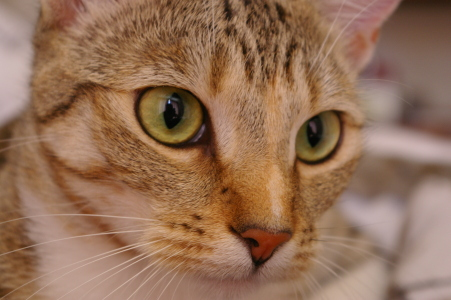
\includegraphics[width=6cm]{figures/cat_full.png}};
% boxes on the photo: (x0, y0, x1, y1) in pixels, the same as in cat_parts.py
\draw[part,blue!80!black]   ({325*\s},{(300-0)*\s})   rectangle ({405*\s},{(300-80)*\s});
\draw[part,red!80!black]    ({130*\s},{(300-80)*\s})  rectangle ({215*\s},{(300-165)*\s});
\draw[part,orange!90!black] ({222*\s},{(300-205)*\s}) rectangle ({307*\s},{(300-290)*\s});
\draw[part,green!50!black]  ({20*\s},{(300-205)*\s})  rectangle ({105*\s},{(300-290)*\s});
% the parts, enlarged
\node[crop,blue!80!black]   (ear)  at (7.6,3.45) {
\includegraphics[width=1.05cm]{figures/cat_ear.png}};
\node[crop,red!80!black]    (eye)  at (7.6,2.15) {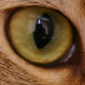
\includegraphics[width=1.05cm]{figures/cat_eye.png}};
\node[crop,orange!90!black] (nose) at (7.6,0.85) {
\includegraphics[width=1.05cm]{figures/cat_nose.png}};
\node[crop,green!50!black]  (whi)  at (7.6,-0.45) {
\includegraphics[width=1.05cm]{figures/cat_whisker.png}};
\draw[dashed,blue!80!black]   ({405*\s},{(300-40)*\s})  -- (ear.west);
\draw[dashed,red!80!black]    ({215*\s},{(300-122)*\s}) -- (eye.west);
\draw[dashed,orange!90!black] ({307*\s},{(300-248)*\s}) -- (nose.west);
\draw[dashed,green!50!black]  ({62*\s},{(300-290)*\s})  -- (whi.west);
\node[right=1mm of ear,font=\small]  (lear)  {귀};
\node[right=1mm of eye,font=\small]  (leye)  {눈};
\node[right=1mm of nose,font=\small] (lnose) {코};
\node[right=1mm of whi,font=\small]  (lwhi)  {수염};
% the whole
\node[draw,rounded corners=4pt,fill=orange!15,font=\bfseries,minimum width=17mm,minimum height=10mm] (cat) at (11.2,1.5) {고양이!};
\foreach \p in {lear,leye,lnose,lwhi} \draw[->,thick,black!60] ([xshift=1mm]\p.east) -- (cat.west);
% the hierarchy
\node[stage] (s1) at (1.9,-2.1) {\textbf{작은 영역}\\에지, 색, 질감\\[1pt]{\scriptsize (앞쪽 합성곱 계층)}};
\node[stage] (s2) at (6.4,-2.1) {\textbf{부분}\\눈, 귀, 코, 수염\\[1pt]{\scriptsize (깊은 합성곱 계층)}};
\node[stage] (s3) at (10.9,-2.1) {\textbf{전체}\\고양이\\[1pt]{\scriptsize (완전연결 계층, Softmax)}};
\draw[->,thick] (s1) -- (s2);
\draw[->,thick] (s2) -- (s3);
\end{tikzpicture}
\end{adjustbox}
\figcap{$13$만 개의 픽셀을 한꺼번에 비교하지 않는다: 부분(귀, 눈, 코, 수염)을 먼저 알아보고, 모아서 ``고양이''로 판단. 각 부분은 \textbf{주변의 좁은 영역}만 보면 된다.}
\end{frame}

\begin{frame}{CNN은 이 과정을 모델링한다}
\begin{itemize}
\item \textbf{좁은 영역씩 본다}: 합성곱 계층의 출력 하나는 입력의 작은 영역 ($3\times3$, $5\times5$)에만 연결
\item \textbf{같은 검출기를 어디에나 쓴다}: ``눈 검출기''는 왼쪽 눈에도 오른쪽 눈에도 $\Rightarrow$ 필터 하나를 모든 위치로 밀며 적용
\item \textbf{단순한 것에서 복잡한 것으로}: 앞쪽 계층은 에지·색, 뒤쪽 계층은 눈·귀 같은 부분, 마지막 완전연결 계층이 ``고양이''를 판단
\end{itemize}
\vskip2mm

\end{frame}

\begin{frame}{전형적인 CNN의 구조}
\centering
\begin{adjustbox}{max width=\linewidth,max totalheight=4.6cm}
\begin{tikzpicture}[>=Latex,scale=0.92,
  fmb/.style={draw=blue!60!black,fill=blue!30,line width=0.5pt},
  fmg/.style={draw=green!60!black,fill=green!30,line width=0.5pt},
  fmy/.style={draw=yellow!60!black,fill=yellow!30,line width=0.5pt},
  fmo/.style={draw=orange!60!black,fill=orange!30,line width=0.5pt},
  kb/.style={draw=red!80!black,thick},
  dl/.style={dashed,thick,black!70},
  nn/.style={draw=blue!60!black,fill=blue!25,circle,minimum size=4mm,inner sep=0pt},
  lab/.style={font=\scriptsize,align=center},
  brc/.style={decorate,decoration={brace,mirror,amplitude=5pt},thick,black!60,text=black}]
% input image and the filter window
\node[inner sep=0pt,draw=black!40] at (0.95,0) {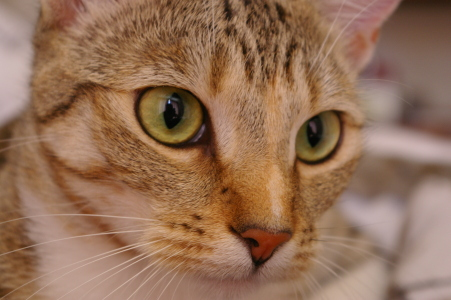
\includegraphics[width=1.9cm]{figures/cat_full.png}};
\draw[kb] (1.15,-0.05) rectangle (1.45,0.25);
% convolution 1: 4 feature maps
\foreach \k in {3,2,1,0} \draw[fmb] ({2.8+\k*0.13},{-0.9+\k*0.13}) rectangle ++(1.8,1.8);
\draw[dl] (1.45,0.25) -- (3.4,0.1);  \draw[dl] (1.45,-0.05) -- (3.4,0.1);
\fill[red!80!black] (3.4,0.1) circle (1.6pt);
\draw[kb] (3.9,-0.45) rectangle ++(0.35,0.35);
% pooling 1: smaller maps, the same number
\foreach \k in {3,2,1,0} \draw[fmg] ({5.6+\k*0.12},{-0.6+\k*0.12}) rectangle ++(1.2,1.2);
\draw[dl] (4.25,-0.1) -- (6.1,-0.2);  \draw[dl] (4.25,-0.45) -- (6.1,-0.2);
\fill[red!80!black] (6.1,-0.2) circle (1.6pt);
\draw[kb] (6.35,0.0) rectangle ++(0.3,0.3);
% convolution 2: more feature maps
\foreach \k in {6,5,...,0} \draw[fmy] ({7.9+\k*0.1},{-0.6+\k*0.1}) rectangle ++(1.2,1.2);
\draw[dl] (6.65,0.3) -- (8.4,0.1);  \draw[dl] (6.65,0.0) -- (8.4,0.1);
\fill[red!80!black] (8.4,0.1) circle (1.6pt);
\draw[kb] (8.7,-0.45) rectangle ++(0.3,0.3);
% pooling 2
\foreach \k in {6,5,...,0} \draw[fmo] ({10.4+\k*0.09},{-0.4+\k*0.09}) rectangle ++(0.8,0.8);
\draw[dl] (9.0,-0.15) -- (10.75,-0.1);  \draw[dl] (9.0,-0.45) -- (10.75,-0.1);
\fill[red!80!black] (10.75,-0.1) circle (1.6pt);
% flatten -> fully connected -> output
\draw[dl] (11.74,0.94) -- (12.48,1.33);  \draw[dl] (11.2,-0.4) -- (12.48,-1.33);
\foreach \i in {0,...,7} \foreach \j in {-2,...,2} \draw[black!25] (12.72,{1.21-\i*0.38}) -- (13.7,{\j*0.6});
\foreach \j in {-2,...,2} \foreach \o in {-1,0,1} \draw[black!25] (13.7,{\j*0.6}) -- (14.8,{\o*0.6});
\foreach \i in {0,...,7} \draw[draw=black!60,fill=black!20] (12.48,{1.33-\i*0.38}) rectangle ++(0.24,-0.24);
\foreach \j in {-2,...,2} \node[nn] at (13.7,{\j*0.6}) {};
\foreach \o in {-1,0,1} \node[nn,fill=orange!40,draw=orange!80!black] at (14.8,{\o*0.6}) {};
\node[anchor=west,font=\scriptsize] at (15.0,0.6)  {고양이 $0.85$};
\node[anchor=west,font=\scriptsize] at (15.0,0)    {개 $0.10$};
\node[anchor=west,font=\scriptsize] at (15.0,-0.6) {새 $0.05$};
% labels
\node[lab] at (3.9,1.75) {합성곱};
\node[lab] at (6.4,1.75) {풀링};
\node[lab] at (8.9,1.75) {합성곱};
\node[lab] at (11.0,1.75) {풀링};
\node[lab] at (15.5,1.85) {출력};
\node[lab] at (0.95,-1.25) {입력 이미지\\{\color{red!80!black}(빨간 상자: 필터)}};
\node[lab] at (3.7,-1.35) {특징 맵};
\node[lab] at (6.2,-1.35) {풀링된\\특징 맵};
\node[lab] at (8.6,-1.35) {특징 맵\\(채널 증가)};
\node[lab] at (10.85,-1.35) {풀링된\\특징 맵};
\node[lab] at (12.6,1.85) {펼치기\\(Flatten)};
\node[lab] at (13.9,1.85) {완전연결\\계층};
% the three stages
\draw[brc] (2.8,-2.4) -- (11.8,-2.4) node[midway,below=5pt,lab,font=\small] {특징 추출 (합성곱 계층 + 풀링 계층)};
\draw[brc] (12.3,-2.4) -- (14.2,-2.4) node[midway,below=5pt,lab,font=\small] {분류};
\draw[brc] (14.5,-2.4) -- (16.4,-2.4) node[midway,below=5pt,lab,font=\small] {확률 (Softmax)};
\end{tikzpicture}
\end{adjustbox}
\raggedright
\small
\begin{itemize}
\item 입력의 작은 영역 $\times$ 필터(빨간 상자, 가중치)의 합 $\to$ 다음 특징 맵의 한 점; \textbf{필터 하나 = 특징 하나를 뽑는 가중치}
\item 합성곱·풀링을 거듭할수록 특징 맵은 \textbf{작아지고}, 개수(채널)는 \textbf{많아진다}
\item 마지막 특징 맵을 펼친 뒤(Flatten) 지금까지 배운 완전연결 계층과 Softmax로 분류
\end{itemize}
\end{frame}

\begin{frame}{완전연결 신경망과 CNN의 계층 구성}
\centering
\begin{adjustbox}{max width=\linewidth,max totalheight=4.2cm}
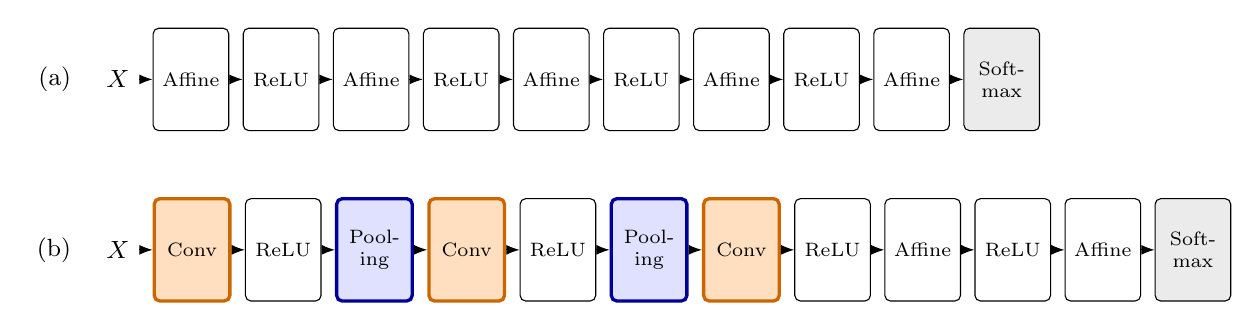
\begin{tikzpicture}[>=Latex,
  lay/.style={draw,rounded corners=2pt,minimum width=9.6mm,minimum height=13mm,
              font=\scriptsize,align=center,inner sep=1pt},
  cv/.style={lay,fill=orange!25,draw=orange!80!black,very thick},
  pl/.style={lay,fill=blue!12,draw=blue!60!black,very thick},
  node distance=1.7mm]
% fully connected
\node[font=\small] (in) {$X$};
\node[lay,right=of in] (a1) {Affine};
\node[lay,right=of a1] (r1) {ReLU};
\node[lay,right=of r1] (a2) {Affine};
\node[lay,right=of a2] (r2) {ReLU};
\node[lay,right=of r2] (a3) {Affine};
\node[lay,right=of a3] (r3) {ReLU};
\node[lay,right=of r3] (a4) {Affine};
\node[lay,right=of a4] (r4) {ReLU};
\node[lay,right=of r4] (a5) {Affine};
\node[lay,right=of a5,fill=black!8] (sm) {Soft-\\max};
\foreach \u/\v in {in/a1,a1/r1,r1/a2,a2/r2,r2/a3,a3/r3,r3/a4,a4/r4,r4/a5,a5/sm}
  \draw[->] (\u) -- (\v);
\node[font=\small,anchor=east] at ([xshift=-2mm]in.west) {(a)};
% CNN
\node[font=\small,below=17mm of in] (in2) {$X$};
\node[cv,right=of in2] (c1) {Conv};
\node[lay,right=of c1] (q1) {ReLU};
\node[pl,right=of q1] (p1) {Pool-\\ing};
\node[cv,right=of p1] (c2) {Conv};
\node[lay,right=of c2] (q2) {ReLU};
\node[pl,right=of q2] (p2) {Pool-\\ing};
\node[cv,right=of p2] (c3) {Conv};
\node[lay,right=of c3] (q3) {ReLU};
\node[lay,right=of q3] (b1) {Affine};
\node[lay,right=of b1] (s1) {ReLU};
\node[lay,right=of s1] (b2) {Affine};
\node[lay,right=of b2,fill=black!8] (sm2) {Soft-\\max};
\foreach \u/\v in {in2/c1,c1/q1,q1/p1,p1/c2,c2/q2,q2/p2,p2/c3,c3/q3,q3/b1,b1/s1,s1/b2,b2/sm2}
  \draw[->] (\u) -- (\v);
\node[font=\small,anchor=east] at ([xshift=-2mm]in2.west) {(b)};
\end{tikzpicture}
\end{adjustbox}
\raggedright
\small
\begin{itemize}
\item (a) 완전연결 신경망(FNN): 인접 계층의 모든 노드가 연결 $\to$ \textbf{Affine} 계층으로 구현
\item (b) CNN: ``Affine $\to$ ReLU'' 대신 ``\textbf{Conv} $\to$ ReLU $\to$ (\textbf{Pooling})'' (풀링은 생략하기도 함)
\item 출력 가까이는 ``Affine $\to$ ReLU'', 마지막은 ``Affine $\to$ Softmax'' $\Rightarrow$ 앞부분은 특징 추출, 뒷부분은 분류
\end{itemize}
\end{frame}

% =================================================
\section{합성곱 계층}
% =================================================

\begin{frame}{완전연결 계층의 문제점}
\begin{itemize}
\item \textbf{데이터의 형상이 무시된다}
  \begin{itemize}
  \item MNIST 이미지는 (채널, 세로, 가로) $=(1,28,28)$인 3차원 데이터
  \item Affine 계층에 넣으려면 $784$개의 값을 한 줄로 펼쳐야 했다
  \end{itemize}
\item 이미지의 \textbf{3차원 모양에 담긴 패턴}
  \begin{itemize}
  \item 공간적으로 가까운 픽셀끼리 값이 비슷하고, 떨어진 픽셀끼리는 관련이 적다
  \item RGB의 세 채널은 서로 밀접하게 관련
  \end{itemize}
\item 완전연결 계층은 모든 입력을 같은 차원의 값으로 취급
  \begin{itemize}
  \item 값은 그대로 남지만 (reshape로 복원 가능), 이웃 관계에 대한 가정이 없다
  \item 모든 이미지의 픽셀을 같은 순서로 섞어도 표현할 수 있는 함수는 같다
  \item 이웃 관계를 처음부터 데이터로 배워야 한다
  \end{itemize}
\end{itemize}
\end{frame}

\begin{frame}{펼치면 드러나지 않는 이웃 관계}
\centering
\begin{adjustbox}{max width=\linewidth,max totalheight=4.6cm}
\begin{tikzpicture}[>=Latex,
  lb/.style={font=\scriptsize\bfseries,inner sep=0pt},
  brc/.style={decorate,decoration={brace,mirror,amplitude=4pt},thick,black!60}]
\def\s{0.4}% cell size of the image (cm)
\def\t{0.3}% cell size of the flattened vector (cm)
% (a) a 7x7 image of the digit 7: white ink on black, as in MNIST
\foreach \r/\row in {0/{0,1,1,1,1,1,0},1/{0,0,0,0,0,1,0},2/{0,0,0,0,1,0,0},3/{0,0,0,1,0,0,0},
                     4/{0,0,0,1,0,0,0},5/{0,0,1,0,0,0,0},6/{0,0,1,0,0,0,0}} {
  \foreach \v [count=\c from 0] in \row {
    \pgfmathtruncatemacro{\g}{85-85*\v}
    \fill[black!\g] ({\c*\s},{-\r*\s}) rectangle ++(\s,-\s);
    \pgfmathtruncatemacro{\i}{\r*7+\c}
    \fill[black!\g] ({\i*\t},-4.0) rectangle ++(\t,-\t);
  }}
\draw[black!40,step=\s] (0,{-7*\s}) grid ({7*\s},0);
% highlighted pixels: A, its right neighbour B, the pixel below C, a far pixel D
\foreach \r/\c/\col/\n in {3/3/red/A,3/4/cyan/B,4/3/green/C,6/6/orange/D} {
  \draw[\col,line width=1.6pt] ({\c*\s},{-\r*\s}) rectangle ++(\s,-\s);
  \node[lb,\col] at ({\c*\s+0.5*\s},{-\r*\s-0.5*\s}) {\n};
  \pgfmathtruncatemacro{\i}{\r*7+\c}
  \draw[\col,line width=1.6pt] ({\i*\t},-4.0) rectangle ++(\t,-\t);
  \node[lb,\col!70!black] at ({\i*\t+0.5*\t},-3.75) {\n};
}
\node[font=\small,align=center] at ({3.5*\s},-3.15) {(a) 이미지 $(7\times7)$};
% (b) the flattened vector
\foreach \k in {1,...,6} \draw[black!70,thick] ({7*\k*\t},-3.9) -- ({7*\k*\t},-4.4);
\draw[black!40] (0,-4.0) rectangle ({49*\t},{-4.0-\t});
\foreach \k in {1,...,7} \node[font=\tiny,black!60] at ({(7*\k-3.5)*\t},-4.5) {\k 행};
\draw[brc] ({24.5*\t},-4.75) -- ({31.5*\t},-4.75) node[midway,below=4pt,font=\scriptsize,text=black] {A와 C: $7$칸 떨어짐};
\node[font=\small] at ({24.5*\t},-5.55) {(b) 한 줄로 펼친 벡터 $(49)$};
\draw[->,thick,black!60] (3.2,-1.4) .. controls (4.6,-1.8) and (5.4,-2.6) .. ({24.5*\t},-3.6)
  node[pos=0.35,right=2pt,font=\scriptsize,black] {펼치기 (reshape)};
% (c) the three channels of a color image
\foreach \x/\y/\col/\ly in {9.9/0.2/blue/-0.1,9.5/-0.2/green/-2.0,9.1/-0.6/red/-2.4} {
  \fill[\col!15] (\x,\y) rectangle ++({5*\s},{-5*\s});
  \draw[\col!60!black,step=\s,shift={(\x,\y)}] (0,{-5*\s}) grid ({5*\s},0);
  \draw[black,line width=1.4pt] ({\x+2*\s},{\y-2*\s}) rectangle ++(\s,-\s);
}
\foreach \xe/\ly/\col/\n in {11.9/-0.1/blue/B,11.5/-1.95/green/G,11.1/-2.4/red/R} {
  \draw[\col!60!black] (\xe,\ly) -- (12.25,\ly);
  \node[font=\small\bfseries,\col!60!black,right] at (12.25,\ly) {\n};
}
\draw[dashed,thick] ({9.1+2.5*\s},{-0.6-2.5*\s}) -- ({9.9+2.5*\s},{0.2-2.5*\s});
\node[font=\small,align=center] at (10.5,-3.15) {(c) 컬러 이미지의 3채널\\[-1pt]{\scriptsize 같은 위치의 R, G, B}};
\end{tikzpicture}
\end{adjustbox}
\raggedright
\small
\begin{itemize}
\item A의 오른쪽 이웃 B는 옆에 남지만, 아래 이웃 C는 $7$칸 (MNIST라면 $28$칸) 떨어진다; (c) 같은 위치의 R, G, B는 한 점의 색
\item 합성곱 계층은 \textbf{형상을 유지}: 입출력 데이터 = \textbf{특징 맵(feature map)} (입력 특징 맵, 출력 특징 맵)
\end{itemize}
\end{frame}

\begin{frame}{합성곱 연산: 채널이 하나인 경우}
\begin{columns}[c,onlytextwidth]
\begin{column}{0.55\textwidth}
\centering
\begin{adjustbox}{scale=1.35,max width=\linewidth}
\begin{tikzpicture}
\numgrid{0}{0}{4}{1,2,3,0,0,1,2,3,3,0,1,2,2,3,0,1}
\node[font=\Large] at (2.55,-1) {$\circledast$};
\numgrid{3.1}{-0.25}{3}{2,0,1,0,1,2,1,0,2}
\node[font=\Large] at (5.15,-1) {$\longrightarrow$};
\numgrid{5.8}{-0.5}{2}{15,16,6,15}
\node[font=\small,below] at (1,-2.1) {입력 데이터};
\node[font=\small,below] at (3.85,-2.1) {필터};
\node[font=\small,below] at (6.3,-2.1) {출력};
\end{tikzpicture}
\end{adjustbox}
\end{column}
\begin{column}{0.43\textwidth}
\small
\begin{itemize}
\item 입력 $(4,4)$, 필터 $(3,3)$ $\to$ 출력 $(2,2)$
\item 필터 = \textbf{커널(kernel)}
\item 필터의 \textbf{윈도우}를 일정 간격으로 이동
\item 각 위치에서 \textbf{대응 원소끼리 곱한 뒤 모두 더함} (곱셈-누산)
\item 필터를 뒤집지 않음: 엄밀히는 상호상관(cross-correlation)이지만 관례상 합성곱
\item 왼쪽 위 $\to$ 오른쪽 아래, 모든 위치에서 반복
\end{itemize}
\end{column}
\end{columns}
\end{frame}

\begin{frame}{합성곱 연산의 계산 순서}
\centering
\begin{adjustbox}{max width=\linewidth,max totalheight=4.4cm}
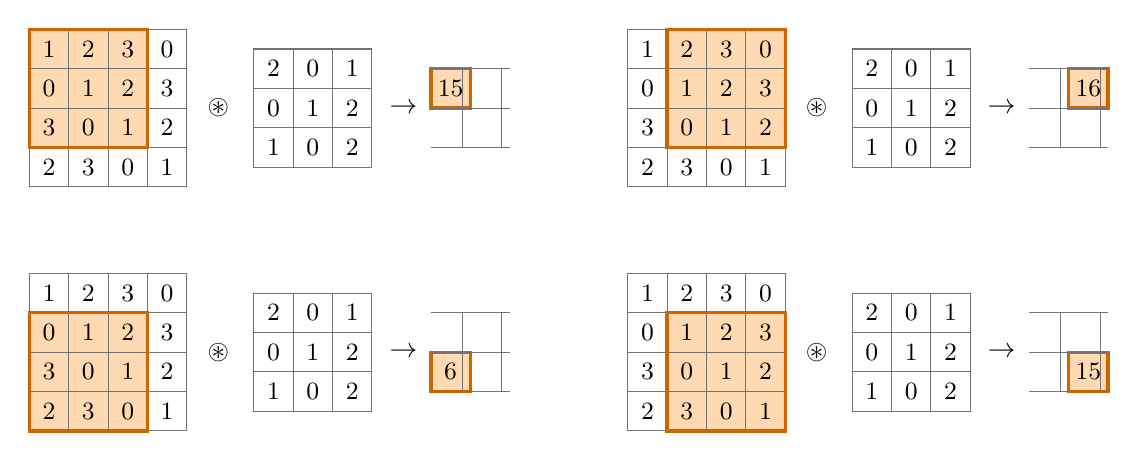
\begin{tikzpicture}
\foreach \oi/\oj/\px/\py/\val in {0/0/0/0/15, 0/1/7.6/0/16, 1/0/0/-3.1/6, 1/1/7.6/-3.1/15} {
  \begin{scope}[shift={(\px,\py)}]
    \fill[orange!30] ({\oj*\cellsz},{-\oi*\cellsz}) rectangle ++({3*\cellsz},{-3*\cellsz});
    \numgrid{0}{0}{4}{1,2,3,0,0,1,2,3,3,0,1,2,2,3,0,1}
    \draw[orange!80!black,very thick] ({\oj*\cellsz},{-\oi*\cellsz}) rectangle ++({3*\cellsz},{-3*\cellsz});
    \node at (2.4,-1) {$\circledast$};
    \numgrid{2.85}{-0.25}{3}{2,0,1,0,1,2,1,0,2}
    \node at (4.75,-1) {$\to$};
    \fill[orange!30] ({5.1+\oj*\cellsz},{-0.5-\oi*\cellsz}) rectangle ++(\cellsz,-\cellsz);
    \draw[orange!80!black,very thick] ({5.1+\oj*\cellsz},{-0.5-\oi*\cellsz}) rectangle ++(\cellsz,-\cellsz);
    \draw[black!55] (5.1,-0.5) grid[step=\cellsz] ++({2*\cellsz},{-2*\cellsz});
    \node[font=\small] at ({5.1+\oj*\cellsz+0.5*\cellsz},{-0.5-\oi*\cellsz-0.5*\cellsz}) {\val};
  \end{scope}
}
\end{tikzpicture}
\end{adjustbox}
\raggedright
\small
\begin{itemize}
\item 첫 위치: $1\cdot2+2\cdot0+3\cdot1+0\cdot0+1\cdot1+2\cdot2+3\cdot1+0\cdot0+1\cdot2=15$
\item 입력 $x$, 필터 $f$ ($FH\times FW$)에 대하여 \quad
$\displaystyle y_{ij}=\sum_{p=0}^{FH-1}\sum_{q=0}^{FW-1}x_{i+p,\,j+q}\,f_{pq}$
\end{itemize}
\end{frame}

\begin{frame}{사람이 설계한 필터: 이미지 처리에서의 특징 추출}
\small
\begin{itemize}
\item 방금 본 계산 (작은 행렬 = \textbf{필터}를 밀며 곱해 더하기)은 CNN 이전부터 이미지 처리에서 써 왔다
\item 어떤 특징을 뽑을지는 필터의 값이 정하고, 그 값은 \textbf{사람이 설계}
\end{itemize}
\vskip2mm
\centering
\footnotesize\renewcommand{\arraystretch}{1.1}
\begin{tabular}{@{}l c p{0.5\textwidth}@{}}
\toprule
필터 & 값 & 하는 일 \\
\midrule
평균 (blur) & $\dfrac{1}{25}\begin{pmatrix}1&\cdots&1\\ \vdots&\ddots&\vdots\\ 1&\cdots&1\end{pmatrix}_{5\times5}$
& 주변 $25$개 픽셀의 평균. 잡음과 세부가 사라지고 흐려진다. \\[4pt]
선명하게 (sharpen) & $\begin{pmatrix}0&-1&0\\-1&5&-1\\0&-1&0\end{pmatrix}$
& 가운데 픽셀과 이웃의 차이를 키운다. 윤곽이 또렷해진다. \\[4pt]
Sobel $x$ & $\begin{pmatrix}-1&0&1\\-2&0&2\\-1&0&1\end{pmatrix}$
& 오른쪽 열 $-$ 왼쪽 열: 가로 방향 밝기 변화, 즉 \textbf{세로 에지}에 반응한다. \\
\bottomrule
\end{tabular}
\end{frame}

\begin{frame}{사람이 설계한 필터 (계속)}
\small
\centering
\footnotesize\renewcommand{\arraystretch}{1.1}
\begin{tabular}{@{}l c p{0.5\textwidth}@{}}
\toprule
필터 & 값 & 하는 일 \\
\midrule
Sobel $y$ & $\begin{pmatrix}-1&-2&-1\\0&0&0\\1&2&1\end{pmatrix}$
& 아래 행 $-$ 위 행: 세로 방향 밝기 변화, 즉 \textbf{가로 에지}에 반응한다. \\[4pt]
Laplacian & $\begin{pmatrix}0&1&0\\1&-4&1\\0&1&0\end{pmatrix}$
& 이웃의 합 $-$ $4\times$가운데 (2계 미분의 근사): 방향에 관계없이 에지에 반응한다. \\[4pt]
엠보싱 (emboss) & $\begin{pmatrix}-2&-1&0\\-1&1&1\\0&1&2\end{pmatrix}$
& 대각선 방향의 밝기 변화를 더해 돋을새김처럼 보이게 한다. \\
\bottomrule
\end{tabular}
\end{frame}

\begin{frame}{왜 이런 필터가 에지에 반응할까?}
\centering
\begin{adjustbox}{scale=1.15,max width=\linewidth,max totalheight=4.2cm}
\begin{tikzpicture}
\numgrid{0}{-0.95}{5}{0,0,0,1,1,0,0,0,1,1,0,0,0,1,1,0,0,0,1,1,0,0,0,1,1}
\node[font=\Large] at (3.05,-0.75) {$\circledast$};
\numgrid{3.5}{0}{3}{-1,0,1,-2,0,2,-1,0,1}
\node[font=\Large] at (5.45,-0.75) {$\to$};
\numgrid{6.0}{0}{3}{0,4,4,0,4,4,0,4,4}
\node[font=\Large] at (3.05,-3.15) {$\circledast$};
\numgrid{3.5}{-2.4}{3}{-1,-2,-1,0,0,0,1,2,1}
\node[font=\Large] at (5.45,-3.15) {$\to$};
\numgrid{6.0}{-2.4}{3}{0,0,0,0,0,0,0,0,0}
\node[font=\small,below] at (1.25,-3.5) {입력 (세로 에지)};
\node[font=\small,right] at (7.6,-0.75) {Sobel $x$: 에지에서 큰 값};
\node[font=\small,right] at (7.6,-3.15) {Sobel $y$: 모두 $0$};
\end{tikzpicture}
\end{adjustbox}
\raggedright
\small
\begin{itemize}
\item 왼쪽 절반 $0$(검정), 오른쪽 절반 $1$(흰색)인 $5\times5$ 이미지; Sobel 원소의 합 $=0$ $\Rightarrow$ 밝기가 고른 곳은 출력 $0$
\item Sobel $x$: $0/1$ 경계가 창 안에 있을 때만 $(0\cdot(-1)+1\cdot1)(1+2+1)=4$; Sobel $y$: 위아래 변화가 없어 모두 $0$
\item 출력 = 그 위치의 이미지 조각이 \textbf{필터의 무늬와 얼마나 닮았는가}
\end{itemize}
\end{frame}

\begin{frame}{사람이 설계한 필터를 사진에 적용하면}
\centering
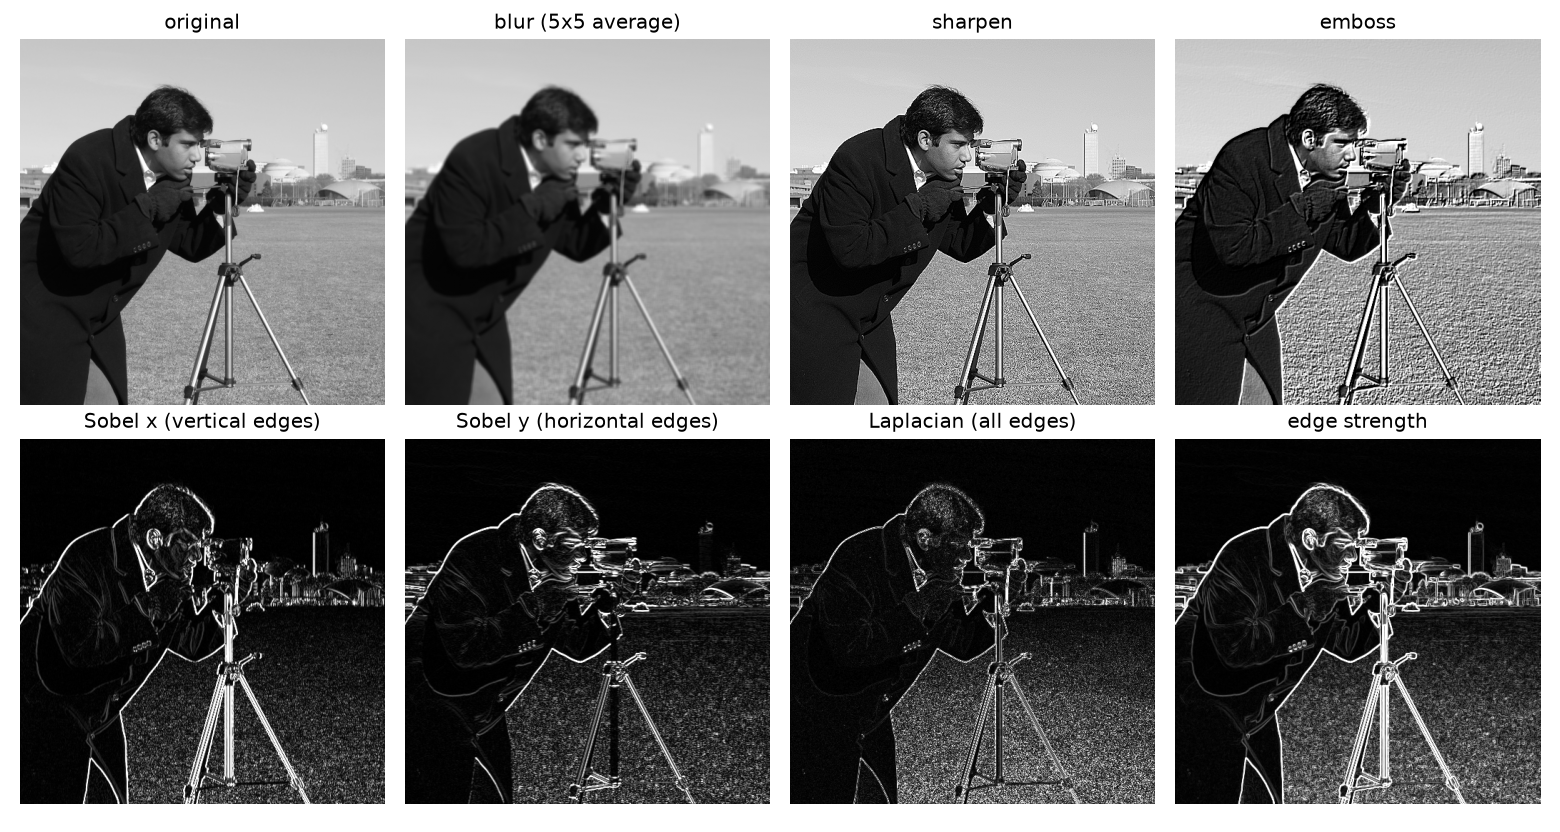
\includegraphics[height=4.8cm]{figures/cnn_classic_filters.png}
\figcap{\texttt{classic\_filters.py} ($512\times512$ 흑백 사진). 위: 원본, 평균, 선명하게, 엠보싱. 아래: Sobel $x$, Sobel $y$, Laplacian, 에지의 세기 $\sqrt{g_x^2+g_y^2}$\\
(에지 필터의 출력은 양수·음수가 모두 나오므로 절댓값; 밝을수록 강한 에지)}
\raggedright
\footnotesize
\begin{itemize}
\item $g_x$, $g_y$ = 같은 위치에서 Sobel $x$, Sobel $y$의 출력 (가로·세로 방향의 밝기 변화량) $\to$ 에지의 세기 $\sqrt{g_x^2+g_y^2}$ = 벡터 $(g_x,g_y)$의 길이: 어느 방향의 에지든 밝게
\end{itemize}
\end{frame}

\begin{frame}{Sobel $x$와 Sobel $y$의 차이 (확대)}
\centering
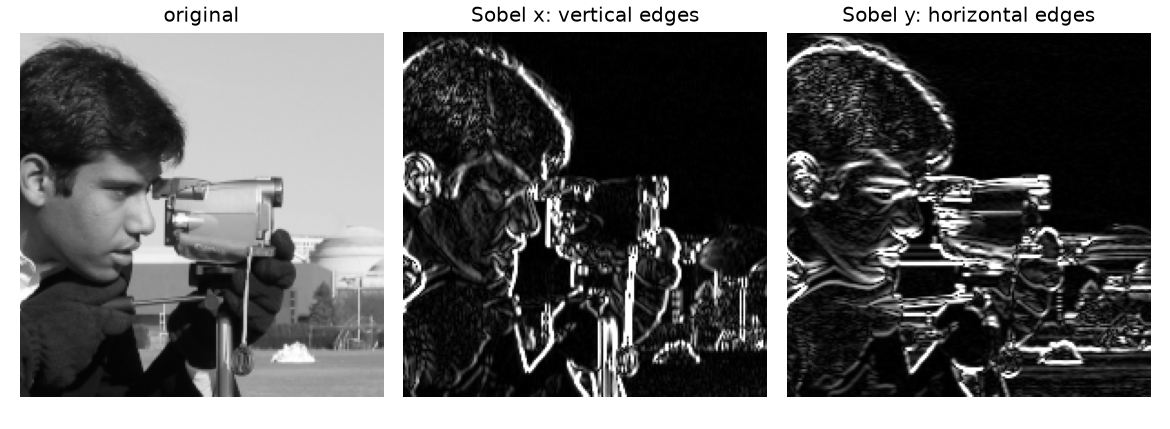
\includegraphics[width=0.95\linewidth]{figures/cnn_classic_filters_zoom.png}
\raggedright
\small
\begin{itemize}
\item Sobel $x$: 삼각대 다리, 얼굴의 옆선처럼 \textbf{세로로 뻗은 경계}가 밝다
\item Sobel $y$: 카메라의 윗면·아랫면, 지평선처럼 \textbf{가로로 뻗은 경계}가 밝다
\item 필터 하나가 이미지에서 \textbf{한 종류의 특징}만 골라낸다
\end{itemize}
\end{frame}

\begin{frame}{사람이 설계한 필터는 지금 어디에 쓰이는가}
\begin{remarkbox}[사람이 설계한 필터는 지금 어디에 쓰이는가]
\footnotesize
딥러닝이 대신한 것은 ``이것이 고양이인가'' 같은 복잡한 인식. 단순하고 목적이 분명한 처리에는 지금도 고정된 필터를 쓴다.
\begin{itemize}
\item \textbf{사진·영상 편집과 카메라}: 흐림 효과, 선명하게, 잡음 제거, 윤곽 보정, 축소 전 블러(앨리어싱 방지)
\item \textbf{고전 컴퓨터 비전}: Canny (가우시안 블러 $\to$ Sobel), Harris 코너, HOG·SIFT (HOG + SVM 보행자 검출)
\item \textbf{산업 현장}: 표면 긁힘 검사, 문서 스캔·OCR 전처리, 차선 인식 (불량 데이터가 적거나 GPU 없는 임베디드)
\item \textbf{딥러닝 안에서}: 데이터 증강, 흐린 사진 걸러내기 (Laplacian 분산), Sobel 에지 손실, BlurPool
\end{itemize}
고정된 필터는 \textbf{데이터가 필요 없고, 해석할 수 있고, 빠르다} — 대신 사람이 수식으로 정의할 수 있는 특징까지만.
\end{remarkbox}
\end{frame}

\begin{frame}{사람이 설계한 필터에서 학습하는 필터로}
\begin{keybox}[사람이 설계한 필터에서 학습하는 필터로]
\begin{itemize}
\item 필터 연산 = \textbf{작은 무늬 검출기}; 출력은 각 위치에서 그 무늬가 얼마나 강한지 담은 2차원 지도, 즉 \textbf{특징 맵}
\item 복잡한 이미지를 분류하려면 어떤 필터를, 어떤 값으로 써야 할지 사람이 정하기 어렵다
\item CNN은 필터의 값을 \textbf{데이터로부터 학습}하는 \textbf{가중치}로 취급 (필터 = 학습 파라미터)
\item 학습된 첫 층의 필터도 Sobel처럼 여러 방향의 에지에 반응하고, 층이 깊어질수록 더 복잡한 무늬를 찾는다
\end{itemize}
\end{keybox}
\end{frame}

\begin{frame}{필터가 가중치이다}
\centering
\begin{adjustbox}{scale=1.25,max width=\linewidth}
\begin{tikzpicture}
\numgrid{0}{0}{4}{1,2,3,0,0,1,2,3,3,0,1,2,2,3,0,1}
\node[font=\Large] at (2.5,-1) {$\circledast$};
\numgrid{3.0}{-0.25}{3}{2,0,1,0,1,2,1,0,2}
\node[font=\Large] at (5.0,-1) {$\to$};
\numgrid{5.5}{-0.5}{2}{15,16,6,15}
\node[font=\Large] at (7.0,-1) {$+$};
\numgrid{7.5}{-0.75}{1}{3}
\node[font=\Large] at (8.5,-1) {$\to$};
\numgrid{9.0}{-0.5}{2}{18,19,9,18}
\node[font=\small,below] at (3.75,-1.9) {필터 (가중치)};
\node[font=\small,below] at (7.75,-1.9) {편향};
\end{tikzpicture}
\end{adjustbox}
\raggedright
\vskip3mm
\begin{itemize}
\item 완전연결 신경망: 가중치 $W$와 편향 $B$
\item CNN: \textbf{필터의 원소가 가중치} $\Rightarrow$ 필터의 값을 학습한다
\item 편향: 필터를 적용한 뒤 \textbf{모든 원소에 같은 값 하나}를 더한다
\end{itemize}
\end{frame}

\begin{frame}{합성곱 계층은 연결을 제한한 완전연결 계층이다}
\small
1차원 입력 $x_1,\ldots,x_6$, 길이 $3$인 필터 $(w_1,w_2,w_3)$, 스트라이드 $1$: \quad $y_j=w_1x_j+w_2x_{j+1}+w_3x_{j+2}$ \ ($j=1,\ldots,4$)
\par\vskip1mm
\centering
\begin{adjustbox}{max width=\linewidth,max totalheight=5.0cm}
\begin{tikzpicture}[
  nd/.style={draw,circle,minimum size=6.5mm,inner sep=0pt,font=\scriptsize,fill=white},
  ca/.style={blue!70!black,thick}, cb/.style={orange!85!black,thick}, cc/.style={green!50!black,thick}]
% (a) fully connected
\begin{scope}
\foreach \i in {1,...,6} \node[nd] (a\i) at (0,{-0.75*\i}) {$x_\i$};
\foreach \j in {1,...,4} \node[nd] (b\j) at (2.6,{-0.75*(\j+1)}) {$y_\j$};
\foreach \i in {1,...,6} \foreach \j in {1,...,4} \draw[black!45] (a\i) -- (b\j);
\node[font=\small,align=center] at (1.3,-5.45) {(a) 완전연결\\가중치 $6\times4=24$개};
\end{scope}
% (b) convolution
\begin{scope}[xshift=4.6cm]
\foreach \i in {1,...,6} \node[nd] (c\i) at (0,{-0.75*\i}) {$x_\i$};
\foreach \j in {1,...,4} \node[nd] (d\j) at (2.6,{-0.75*(\j+1)}) {$y_\j$};
\foreach \j [evaluate=\j as \ja using int(\j+1), evaluate=\j as \jb using int(\j+2)] in {1,...,4} {
  \draw[ca] (c\j) -- (d\j);
  \draw[cb] (c\ja) -- (d\j);
  \draw[cc] (c\jb) -- (d\j);
}
\node[font=\small,align=center] at (1.3,-5.45) {(b) 합성곱\\가중치 $3$개 (색이 같으면 같은 값)};
\end{scope}
% (c) the weight matrix of (b)
\begin{scope}[xshift=9.4cm,yshift=-1.0cm]
\def\mc{0.52}
\foreach \r in {0,...,5} \foreach \c in {0,...,3} \draw[black!35] ({\c*\mc},{-\r*\mc}) rectangle ++(\mc,-\mc);
\foreach \c in {0,...,3} {
  \pgfmathtruncatemacro{\ra}{\c}\pgfmathtruncatemacro{\rb}{\c+1}\pgfmathtruncatemacro{\rc}{\c+2}
  \fill[blue!20] ({\c*\mc},{-\ra*\mc}) rectangle ++(\mc,-\mc); \node[font=\scriptsize,blue!70!black] at ({(\c+0.5)*\mc},{-(\ra+0.5)*\mc}) {$w_1$};
  \fill[orange!25] ({\c*\mc},{-\rb*\mc}) rectangle ++(\mc,-\mc); \node[font=\scriptsize,orange!85!black] at ({(\c+0.5)*\mc},{-(\rb+0.5)*\mc}) {$w_2$};
  \fill[green!20] ({\c*\mc},{-\rc*\mc}) rectangle ++(\mc,-\mc); \node[font=\scriptsize,green!50!black] at ({(\c+0.5)*\mc},{-(\rc+0.5)*\mc}) {$w_3$};
}
\foreach \r in {0,...,5} \foreach \c in {0,...,3} \draw[black!35] ({\c*\mc},{-\r*\mc}) rectangle ++(\mc,-\mc);
\node[font=\small,left] at (-0.05,{-3*\mc}) {$W=$};
\node[font=\small,align=center] at ({2*\mc},-4.45) {(c) (b)의 가중치 행렬 $(6\times4)$\\빈칸은 $0$};
\end{scope}
\end{tikzpicture}
\end{adjustbox}
\figcap{$Y=XW$로 쓰면 합성곱은 $W$의 대부분이 $0$이고 같은 값이 대각선을 따라 반복되는 특별한 완전연결 계층}
\end{frame}

\begin{frame}{완전연결 계층 + 두 가지 규칙 = 합성곱 계층}
\begin{itemize}
\item \textbf{국소 연결 (sparse connectivity)}
  \begin{itemize}
  \item $y_j$는 \textbf{공간적으로 인접한} $x_j,x_{j+1},x_{j+2}$에만 연결 $\to$ 이 영역이 $y_j$의 \textbf{수용 영역}
  \item 이미지의 기하 구조(가까운 픽셀끼리 관련이 깊다)를 연결 방식에 반영
  \end{itemize}
\item \textbf{가중치 공유 (parameter sharing)}
  \begin{itemize}
  \item 모든 출력 노드가 \textbf{같은 가중치} $(w_1,w_2,w_3)$ $\to$ 무늬가 어디에 있든 같은 방식으로 찾는다
  \end{itemize}
\item $W$: 각 열에 $w_1,w_2,w_3$이 한 칸씩 내려가며 놓이는 \textbf{띠 모양 행렬}
\item 2차원 예: MNIST $(28\times28)$, $5\times5$ 필터 하나 $\to$ $24\times24$
  \begin{itemize}
  \item 완전연결: $784\times576=451584$개 \quad vs. \quad 합성곱: $\mathbf{25}$개
  \end{itemize}
\end{itemize}
\vskip1mm
{\footnotesize\color{black!60} 참고: Goodfellow, Bengio, Courville, \emph{Deep Learning} 9장 (sparse interactions, parameter sharing)}
\end{frame}

\begin{frame}[fragile]{코드로 확인하기: \texttt{conv2d\_naive} (\texttt{conv\_basics.py})}
\begin{lstlisting}
def conv2d_naive(x, f, stride=1, pad=0):
    """2-D convolution of one image x (H, W) with one filter f (FH, FW), with loops"""
    x = np.pad(x, pad)                                  # zeros around the image
    FH, FW = f.shape
    OH = (x.shape[0] - FH) // stride + 1
    OW = (x.shape[1] - FW) // stride + 1
    y = np.zeros((OH, OW))
    for i in range(OH):
        for j in range(OW):
            window = x[i * stride:i * stride + FH, j * stride:j * stride + FW]
            y[i, j] = np.sum(window * f)                # multiply elementwise, then add
    return y
\end{lstlisting}
\begin{columns}[T,onlytextwidth]
\begin{column}{0.48\textwidth}
\begin{lstlisting}[language={}]
convolution (4x4 input, 3x3 filter):
 [[15. 16.]
 [ 6. 15.]]
\end{lstlisting}
\end{column}
\begin{column}{0.48\textwidth}
\begin{lstlisting}[language={}]
with bias 3:
 [[18. 19.]
 [ 9. 18.]]
\end{lstlisting}
\end{column}
\end{columns}
\end{frame}

\begin{frame}{패딩 (padding)}
\begin{columns}[c,onlytextwidth]
\begin{column}{0.58\textwidth}
\centering
\begin{adjustbox}{scale=1.1,max width=\linewidth}
\begin{tikzpicture}
\fill[black!8] (0,0) rectangle ({6*\cellsz},{-6*\cellsz});
\numgrid{0}{0}{6}{0,0,0,0,0,0,0,1,2,3,0,0,0,0,1,2,3,0,0,3,0,1,2,0,0,2,3,0,1,0,0,0,0,0,0,0}
\draw[very thick] (\cellsz,-\cellsz) rectangle ({5*\cellsz},{-5*\cellsz});
\node[font=\Large] at (3.45,-1.5) {$\circledast$};
\numgrid{4.0}{-0.75}{3}{2,0,1,0,1,2,1,0,2}
\node[font=\Large] at (6.05,-1.5) {$\longrightarrow$};
\numgrid{6.7}{-0.5}{4}{7,12,10,2,4,15,16,10,10,6,15,6,8,10,4,3}
\node[font=\small,below] at (1.5,-3.1) {$(4,4)$ 입력 + 패딩 $1$};
\node[font=\small,below] at (4.75,-3.1) {$(3,3)$ 필터};
\node[font=\small,below] at (7.7,-3.1) {$(4,4)$ 출력};
\end{tikzpicture}
\end{adjustbox}
\end{column}
\begin{column}{0.4\textwidth}
\small
\begin{itemize}
\item 합성곱 전에 입력 주변을 특정 값(보통 $0$)으로 채움
\item 패딩 없음: $(4,4)\to(2,2)$\\ 패딩 $1$: $(4,4)\to(4,4)$
\item 주로 \textbf{출력 크기 조정}: 깊은 network에서 크기가 계속 줄어 $1$이 되는 것을 막음
\item 가장자리 픽셀의 정보도 더 반영
\end{itemize}
\end{column}
\end{columns}
\end{frame}

\begin{frame}{스트라이드 (stride)}
\begin{columns}[c,onlytextwidth]
\begin{column}{0.58\textwidth}
\centering
\begin{adjustbox}{scale=1.1,max width=\linewidth}
\begin{tikzpicture}
\fill[orange!30] (0,0) rectangle ({3*\cellsz},{-3*\cellsz});
\fill[blue!15] ({2*\cellsz},0) rectangle ({5*\cellsz},{-3*\cellsz});
\fill[orange!55!blue!30] ({2*\cellsz},0) rectangle ({3*\cellsz},{-3*\cellsz});
\draw[black!55] (0,0) grid[step=\cellsz] ({7*\cellsz},{-7*\cellsz});
\draw[orange!80!black,very thick] (0,0) rectangle ({3*\cellsz},{-3*\cellsz});
\draw[blue!70!black,very thick,densely dashed] ({2*\cellsz},0) rectangle ({5*\cellsz},{-3*\cellsz});
\draw[->,thick] (0.75,0.35) -- node[above,font=\small] {스트라이드 $2$} (1.75,0.35);
\node[font=\Large] at (4.2,-1.75) {$\circledast$};
\draw[black!55] (4.75,-1) grid[step=\cellsz] ++({3*\cellsz},{-3*\cellsz});
\node[font=\Large] at (7,-1.75) {$\longrightarrow$};
\fill[orange!30] (7.6,-1) rectangle ++(\cellsz,-\cellsz);
\fill[blue!15] ({7.6+\cellsz},-1) rectangle ++(\cellsz,-\cellsz);
\draw[black!55] (7.6,-1) grid[step=\cellsz] ++({3*\cellsz},{-3*\cellsz});
\node[font=\small,below] at (1.75,-3.6) {$(7,7)$ 입력};
\node[font=\small,below] at (5.5,-3.6) {$(3,3)$ 필터};
\node[font=\small,below] at (8.35,-3.6) {$(3,3)$ 출력};
\end{tikzpicture}
\end{adjustbox}
\end{column}
\begin{column}{0.4\textwidth}
\small
\begin{itemize}
\item 필터를 적용하는 위치의 간격
\item 지금까지는 스트라이드 $1$; 스트라이드 $2$이면 윈도우가 두 칸씩 이동
\item $7\times7$, $3\times3$ 필터:\\ 스트라이드 $1\to(5,5)$,\\ 스트라이드 $2\to(3,3)$
\item 스트라이드 $\uparrow$ $\Rightarrow$ 출력 $\downarrow$,\\ 패딩 $\uparrow$ $\Rightarrow$ 출력 $\uparrow$
\end{itemize}
\end{column}
\end{columns}
\end{frame}

\begin{frame}{합성곱의 출력 크기}
입력 $(H,W)$, 필터 $(FH,FW)$, 패딩 $P$, 스트라이드 $S$일 때 출력 $(OH,OW)$:
\begin{keybox}[합성곱의 출력 크기]
\[
OH=\left\lfloor\frac{H+2P-FH}{S}\right\rfloor+1,\qquad OW=\left\lfloor\frac{W+2P-FW}{S}\right\rfloor+1
\]
\end{keybox}
\begin{itemize}
\item 입력 $(4,4)$, $P=1$, $S=1$, 필터 $(3,3)$: $OH=\frac{4+2-3}{1}+1=4$
\item 입력 $(7,7)$, $P=0$, $S=2$, 필터 $(3,3)$: $OH=\frac{7+0-3}{2}+1=3$
\item 입력 $(28,31)$, $P=2$, $S=3$, 필터 $(5,5)$: $OH=\frac{28+4-5}{3}+1=10$, $OW=\frac{31+4-5}{3}+1=11$
\item $\lfloor\cdot\rfloor$ = 내림: 남는 부분에는 필터를 놓지 않는다 (예: $H=8$, $FH=3$, $S=2$ $\to$ $\lfloor 5/2\rfloor+1=3$). 코드의 \texttt{//}, PyTorch도 같다
\end{itemize}
\end{frame}

\begin{frame}{3차원 데이터의 합성곱}
\begin{columns}[c,onlytextwidth]
\begin{column}{0.5\textwidth}
\centering
\begin{adjustbox}{scale=1.2,max width=\linewidth}
\begin{tikzpicture}
\foreach \c/\col in {2/blue,1/green!60!black,0/orange} {
  \begin{scope}[shift={({0.3*\c},{0.3*\c})}]
    \filldraw[fill=\col!15,draw=black!60] (0,0) rectangle ({4*\cellsz},{-4*\cellsz});
    \draw[black!40] (0,0) grid[step=\cellsz] ({4*\cellsz},{-4*\cellsz});
  \end{scope}
  \begin{scope}[shift={({3.3+0.3*\c},{-0.25+0.3*\c})}]
    \filldraw[fill=\col!15,draw=black!60] (0,0) rectangle ({3*\cellsz},{-3*\cellsz});
    \draw[black!40] (0,0) grid[step=\cellsz] ({3*\cellsz},{-3*\cellsz});
  \end{scope}
}
\node[font=\Large] at (2.75,-1) {$\circledast$};
\node[font=\Large] at (5.6,-1) {$\longrightarrow$};
\filldraw[fill=black!8,draw=black!60] (6.3,-0.5) rectangle ++({2*\cellsz},{-2*\cellsz});
\draw[black!40] (6.3,-0.5) grid[step=\cellsz] ++({2*\cellsz},{-2*\cellsz});
\node[font=\small,below,align=center] at (1.3,-2.15) {입력 데이터\\(채널 $3$개, $4\times4$)};
\node[font=\small,below,align=center] at (4.1,-2.15) {필터\\(채널 $3$개, $3\times3$)};
\node[font=\small,below,align=center] at (6.8,-2.15) {출력\\($2\times2$, 채널 $1$개)};
\end{tikzpicture}
\end{adjustbox}
\end{column}
\begin{column}{0.48\textwidth}
\small
\begin{itemize}
\item 이미지는 세로·가로에 \textbf{채널}까지 3차원 (컬러는 RGB $3$채널)
\item \textbf{채널마다} 입력과 필터의 합성곱 $\to$ 결과를 \textbf{모두 더해} 하나의 출력
\end{itemize}
\begin{keybox}[3차원 합성곱의 규칙]
\footnotesize
\begin{itemize}
\item 입력의 채널 수 $=$ 필터의 채널 수
\item 필터 크기 $(FH,FW)$는 자유, 단 모든 채널이 같은 크기
\item 채널 $C$개 입력 $\circledast$ 필터 하나 $\to$ \textbf{채널 $1$개}
\end{itemize}
\vskip-2mm
\[
y_{ij}=\sum_{c=1}^{C}\sum_{p}\sum_{q}x_{c,\,i+p,\,j+q}\,f_{c,\,p,\,q}+b
\]
\end{keybox}
\end{column}
\end{columns}
\end{frame}

\begin{frame}{블록으로 생각하기}
\centering
\begin{adjustbox}{scale=1.35,max width=\linewidth}
\begin{tikzpicture}
\cuboid{0}{0}{1.6}{1.6}{0.9}{blue}
\node[font=\small,below] at (0.8,-0.05) {$(C,H,W)$};
\node[font=\small] at (2.45,0.8) {$\circledast$};
\cuboid{2.9}{0.35}{0.9}{0.9}{0.9}{blue}
\node[font=\small,below] at (3.35,0.3) {$(C,FH,FW)$};
\node[font=\small] at (4.75,0.8) {$\longrightarrow$};
\cuboid{5.3}{0.2}{1.2}{1.2}{0.12}{orange}
\node[font=\small,below] at (5.9,0.15) {$(1,OH,OW)$};
\node[font=\small,anchor=west] at (7.3,0.8) {필터 $1$개 $\Rightarrow$ 특징 맵 $1$장};
\end{tikzpicture}
\end{adjustbox}
\raggedright
\vskip4mm
\begin{itemize}
\item 데이터와 필터를 직육면체 \textbf{블록}으로 생각한다
\item 3차원 데이터의 shape: (채널, 높이, 너비) $=(C,H,W)$, \ 필터: $(C,FH,FW)$
\item 필터 $1$개 $\to$ 출력 $(1,OH,OW)$: 다음 계층에 넘길 정보가 너무 적다
\end{itemize}
\end{frame}

\begin{frame}{필터를 $FN$개 쓰는 합성곱 계층}
\centering
\begin{adjustbox}{scale=1.15,max width=\linewidth}
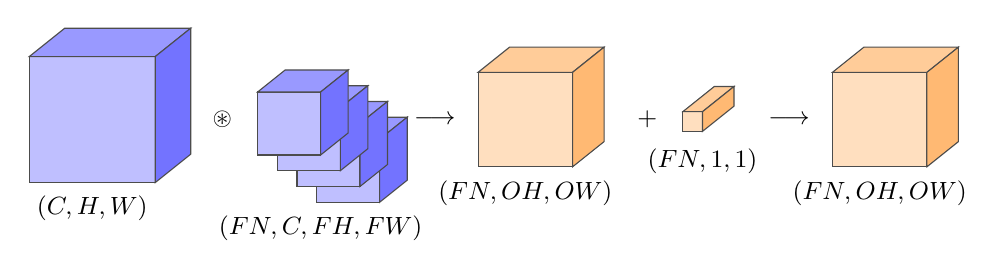
\begin{tikzpicture}
\cuboid{0}{0}{1.6}{1.6}{0.9}{blue}
\node[font=\small,below] at (0.8,-0.05) {$(C,H,W)$};
\node[font=\small] at (2.45,0.8) {$\circledast$};
\foreach \k in {3,2,1,0} {\cuboid{2.9+0.25*\k}{0.35-0.2*\k}{0.8}{0.8}{0.7}{blue}}
\node[font=\small,below] at (3.7,-0.3) {$(FN,C,FH,FW)$};
\node[font=\small] at (5.15,0.8) {$\longrightarrow$};
\cuboid{5.7}{0.2}{1.2}{1.2}{0.8}{orange}
\node[font=\small,below] at (6.3,0.15) {$(FN,OH,OW)$};
\node[font=\small] at (7.85,0.8) {$+$};
\cuboid{8.3}{0.65}{0.25}{0.25}{0.8}{orange}
\node[font=\small,below] at (8.55,0.55) {$(FN,1,1)$};
\node[font=\small] at (9.65,0.8) {$\longrightarrow$};
\cuboid{10.2}{0.2}{1.2}{1.2}{0.8}{orange}
\node[font=\small,below] at (10.8,0.15) {$(FN,OH,OW)$};
\end{tikzpicture}
\end{adjustbox}
\raggedright
\vskip4mm
\begin{itemize}
\item 필터 $FN$개 $\to$ 출력 특징 맵 $FN$장: $(FN,OH,OW)$ 블록
\item 합성곱 계층의 필터(가중치)는 \textbf{4차원} $(FN,C,FH,FW)$
\item 편향은 필터(출력 채널)마다 하나씩 $FN$개: shape $(FN,1,1)$로 보면 broadcast로 더해진다
\end{itemize}
\end{frame}

\begin{frame}{왜 합성곱인가: 가중치 공유}
\begin{thinkbox}[왜 합성곱인가: 가중치 공유]
\begin{itemize}
\item \textbf{같은 필터를 이미지의 모든 위치에 적용} (weight sharing)
  \begin{itemize}
  \item 세로 획 필터 하나가 왼쪽 위의 세로 획도, 오른쪽 아래의 세로 획도 똑같이 찾는다
  \end{itemize}
\item 매개변수가 아주 적다: MNIST $(1,28,28)$ $\to$ 출력 $(30,24,24)$
  \begin{itemize}
  \item 완전연결 계층: $784\times(30\cdot24\cdot24)=784\times17280\approx1350$만 개의 가중치
  \item 합성곱 계층 ($5\times5$ 필터 $30$개): $30\times1\times5\times5=\mathbf{750}$개 가중치 $+$ $30$개 편향
  \end{itemize}
\item 각 출력 원소는 입력의 $5\times5$ 영역만 본다 (\textbf{국소 연결})
\item 이 두 성질이 이미지의 구조에 잘 맞는다
\end{itemize}
\end{thinkbox}
\end{frame}

\begin{frame}{배치 처리}
\centering
\begin{adjustbox}{max width=\linewidth,max totalheight=3.6cm}
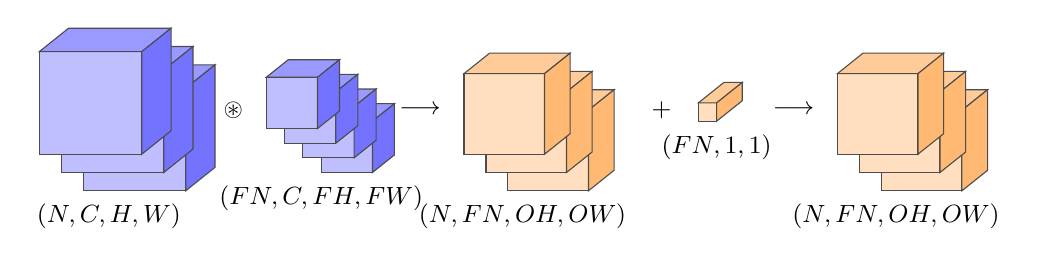
\begin{tikzpicture}[x=0.93cm,y=0.93cm]
\foreach \k in {2,1,0} {\cuboid{0.3*\k}{-0.25*\k}{1.4}{1.4}{0.8}{blue}}
\node[font=\small,below] at (0.95,-0.55) {$(N,C,H,W)$};
\node[font=\small] at (2.65,0.6) {$\circledast$};
\foreach \k in {3,2,1,0} {\cuboid{3.1+0.25*\k}{0.35-0.2*\k}{0.7}{0.7}{0.6}{blue}}
\node[font=\small,below] at (3.85,-0.3) {$(FN,C,FH,FW)$};
\node[font=\small] at (5.2,0.6) {$\longrightarrow$};
\foreach \k in {2,1,0} {\cuboid{5.8+0.3*\k}{-0.25*\k}{1.1}{1.1}{0.7}{orange}}
\node[font=\small,below] at (6.6,-0.55) {$(N,FN,OH,OW)$};
\node[font=\small] at (8.5,0.6) {$+$};
\cuboid{9.0}{0.45}{0.25}{0.25}{0.7}{orange}
\node[font=\small,below] at (9.25,0.4) {$(FN,1,1)$};
\node[font=\small] at (10.3,0.6) {$\longrightarrow$};
\foreach \k in {2,1,0} {\cuboid{10.9+0.3*\k}{-0.25*\k}{1.1}{1.1}{0.7}{orange}}
\node[font=\small,below] at (11.7,-0.55) {$(N,FN,OH,OW)$};
\end{tikzpicture}
\end{adjustbox}
\raggedright
\vskip3mm
\begin{itemize}
\item 완전연결 계층의 미니배치처럼, 합성곱 계층도 \textbf{배치 처리}
\item 데이터를 \textbf{4차원} (데이터 수, 채널, 높이, 너비) $=(N,C,H,W)$로 저장
  \begin{itemize}
  \item 미니배치 크기를 $N$으로 표기 (높이 $H$와 혼동 방지)
  \end{itemize}
\item 4차원 데이터 하나가 흐를 때마다 $N$개에 대한 합성곱이 한 번에 이루어진다
\end{itemize}
\end{frame}

% =================================================
\section{풀링 계층}
% =================================================

\begin{frame}{최대 풀링 (max pooling)}
\begin{columns}[c,onlytextwidth]
\begin{column}{0.45\textwidth}
\centering
\begin{adjustbox}{scale=1.45,max width=\linewidth}
\begin{tikzpicture}
\fill[orange!30] (0,0) rectangle ({2*\cellsz},{-2*\cellsz});
\fill[blue!15] ({2*\cellsz},0) rectangle ({4*\cellsz},{-2*\cellsz});
\fill[green!20] (0,{-2*\cellsz}) rectangle ({2*\cellsz},{-4*\cellsz});
\fill[black!10] ({2*\cellsz},{-2*\cellsz}) rectangle ({4*\cellsz},{-4*\cellsz});
\numgrid{0}{0}{4}{1,2,1,0,0,1,2,3,3,0,1,2,2,4,0,1}
\draw[very thick] (0,0) rectangle ({4*\cellsz},{-4*\cellsz});
\draw[very thick] ({2*\cellsz},0) -- ({2*\cellsz},{-4*\cellsz});
\draw[very thick] (0,{-2*\cellsz}) -- ({4*\cellsz},{-2*\cellsz});
\node[font=\Large] at (3,-1) {$\longrightarrow$};
\fill[orange!30] (3.8,-0.5) rectangle ++(\cellsz,-\cellsz);
\fill[blue!15] ({3.8+\cellsz},-0.5) rectangle ++(\cellsz,-\cellsz);
\fill[green!20] (3.8,{-0.5-\cellsz}) rectangle ++(\cellsz,-\cellsz);
\fill[black!10] ({3.8+\cellsz},{-0.5-\cellsz}) rectangle ++(\cellsz,-\cellsz);
\numgrid{3.8}{-0.5}{2}{2,3,4,2}
\node[font=\small,below] at (1,-2.1) {입력 $(4,4)$};
\node[font=\small,below] at (4.3,-2.1) {출력 $(2,2)$};
\end{tikzpicture}
\end{adjustbox}
\end{column}
\begin{column}{0.52\textwidth}
\small
\begin{itemize}
\item \textbf{풀링}: 세로·가로 방향의 공간을 줄이는 연산
\item $2\times2$ 최대 풀링, 스트라이드 $2$: $2\times2$ 영역마다 \textbf{가장 큰 원소} 하나
\item 윈도우 크기와 스트라이드는 보통 같게 (윈도우 $3\times3$이면 스트라이드 $3$)
\item 영역의 평균을 내는 \textbf{평균 풀링}도 있지만, 이미지 인식에서는 주로 최대 풀링
\item \texttt{pool = Pooling(2, 2)} $\to$ \texttt{[[2. 3.] [4. 2.]]}
\end{itemize}
\end{column}
\end{columns}
\end{frame}

\begin{frame}{풀링 계층의 특징}
\begin{keybox}[풀링 계층의 특징]
\begin{itemize}
\item \textbf{학습해야 할 매개변수가 없다}
  \begin{itemize}
  \item 영역에서 최댓값(또는 평균)을 취하는 명확한 처리일 뿐
  \end{itemize}
\item \textbf{채널 수가 변하지 않는다}
  \begin{itemize}
  \item 채널마다 독립적으로 계산: $(N,C,H,W)\to(N,C,OH,OW)$
  \end{itemize}
\item \textbf{입력의 작은 변화에 영향을 적게 받는다 (robust)}
  \begin{itemize}
  \item 입력이 한두 칸 이동해도 영역 안의 최댓값은 그대로인 경우가 많다
  \item 시각 피질의 \textbf{복합 세포}와 같은 역할
  \end{itemize}
\end{itemize}
\end{keybox}
\end{frame}

% =================================================
\section{합성곱 / 풀링 계층 구현하기}
% =================================================

\begin{frame}{구현 파일}
\begin{itemize}
\item 합성곱·풀링 계층도 \texttt{forward}와 \texttt{backward}를 가진 \textbf{클래스}로 구현
\item Affine, ReLU, Softmax 계층은 지난 시간의 \texttt{layers.py}를 그대로 사용
\end{itemize}
\vskip2mm
\centering
\small
\begin{tabular}{@{}>{\raggedright\arraybackslash}p{0.36\textwidth}>{\raggedright\arraybackslash}p{0.6\textwidth}@{}}
\toprule
파일 & 내용 \\
\midrule
\texttt{conv\_layers.py} & \texttt{im2col}, \texttt{col2im}, \texttt{Convolution}, \texttt{Pooling}, \texttt{Flatten}, \texttt{SimpleConvNet} \\
\texttt{layers.py}, \texttt{optimizers.py}, \texttt{mnist\_data.py} & 지난 시간의 모듈 (그대로 복사) \\[2pt]
\texttt{cat\_parts.py} & 도입부의 고양이 사진과 부분 그림 \\
\texttt{classic\_filters.py} & 사람이 설계한 필터 (평균, Sobel, Laplacian 등)를 흑백 사진에 적용 \\
\texttt{conv\_basics.py} & 이 노트의 예제, im2col 확인과 속도 비교, gradient 확인 \\
\texttt{mnist\_cnn.py} & SimpleConvNet으로 MNIST 학습, 필터와 특징 맵 시각화 \\
\texttt{mnist\_cnn\_torch.py} & 같은 network를 PyTorch로 \\
\bottomrule
\end{tabular}
\end{frame}

\begin{frame}[fragile]{4차원 배열}
\begin{itemize}
\item 계층 사이를 흐르는 데이터: 4차원 배열 $(N,C,H,W)$
\item 높이 $28$, 너비 $28$, 채널 $1$인 데이터 $10$개 $\to$ shape $(10,1,28,28)$
\end{itemize}
\begin{lstlisting}[language={}]
>>> x = np.random.rand(10, 1, 28, 28)
>>> x[0].shape         # the first image: (1, 28, 28)
>>> x[0, 0].shape      # its first channel: (28, 28)
\end{lstlisting}
\begin{itemize}
\item 지금까지 MNIST는 $(N,784)$ $\to$ CNN에서는 \texttt{reshape}으로 모양을 되살려 입력 (\texttt{mnist\_cnn.py})
\end{itemize}
\begin{lstlisting}
x_train = x_train.reshape(-1, 1, 28, 28)   # (N, 784) -> (N, 1, 28, 28)
\end{lstlisting}
\end{frame}

\begin{frame}{im2col로 데이터 전개하기}
\begin{itemize}
\item \texttt{conv2d\_naive}처럼 반복문으로 구현하면: 데이터 $N$개 $\times$ 필터 $FN$개 $\times$ 출력 위치 $OH\times OW$ $\to$ \texttt{for} 문이 겹겹이 (numpy에서 느림)
\item \textbf{im2col} (image to column): 입력을 필터 적용에 좋게 \textbf{2차원 행렬로 펼친다}
\end{itemize}
\begin{keybox}[im2col의 아이디어]
필터가 방문하는 위치 하나마다, 그 위치의 입력 영역 $(C,FH,FW)$을 \textbf{한 행}으로 펼친다.
\begin{itemize}
\item 입력 $(N,C,H,W)$ $\xrightarrow{\text{im2col}}$ 행렬 $(N\cdot OH\cdot OW,\ C\cdot FH\cdot FW)$
\item 필터 $(FN,C,FH,FW)$ $\xrightarrow{\text{reshape}}$ 필터 하나를 \textbf{한 열}로: $(C\cdot FH\cdot FW,\ FN)$
\item 합성곱 $=$ 두 행렬의 곱 $+$ 편향: $(N\cdot OH\cdot OW,\ FN)$ $\xrightarrow{\text{reshape}}$ $(N,FN,OH,OW)$
\end{itemize}
\end{keybox}
\end{frame}

\begin{frame}{im2col을 이용한 합성곱}
\centering
\begin{adjustbox}{max width=\linewidth,max totalheight=3.8cm}
\begin{tikzpicture}[>=Latex]
% input with two windows
\cuboid{0}{0}{1.8}{1.8}{0.6}{blue}
\filldraw[fill=orange!50,draw=orange!80!black,thick] (0,1.8) rectangle ++(0.9,-0.9);
\filldraw[fill=green!40,draw=green!50!black,thick] (0.45,1.8) rectangle ++(0.9,-0.9);
\node[font=\scriptsize] at (0.3,1.1) {\ding{172}};
\node[font=\scriptsize] at (1.2,1.1) {\ding{173}};
\node[font=\small,below] at (0.9,-0.05) {입력 $(C,H,W)$};
\draw[->,thick] (2.5,0.8) -- node[above,font=\small] {im2col} (3.5,0.8);
% the column matrix: one row per filter position
\fill[orange!50] (3.7,2.0) rectangle (5.7,1.75);
\fill[green!40] (3.7,1.75) rectangle (5.7,1.5);
\draw[thick] (3.7,2.0) rectangle (5.7,-0.4);
\node[font=\scriptsize,anchor=east] at (3.65,1.875) {\ding{172}};
\node[font=\scriptsize,anchor=east] at (3.65,1.625) {\ding{173}};
\node[font=\small] at (4.7,0.6) {$\vdots$};
\node[font=\small,below,align=center] at (4.7,-0.45) {$(OH\cdot OW,$\\$C\cdot FH\cdot FW)$};
% the filters: one column per filter
\node[font=\Large] at (6.05,0.8) {$\cdot$};
\fill[blue!25] (6.4,2.0) rectangle (6.7,-0.4);
\fill[blue!45] (6.7,2.0) rectangle (7.0,-0.4);
\draw[thick] (6.4,2.0) rectangle (7.6,-0.4);
\node[font=\small,below,align=center] at (7.0,-0.45) {$(C\cdot FH\cdot FW,$\\$FN)$};
\node[font=\Large] at (8.1,0.8) {$=$};
\fill[orange!50] (8.6,2.0) rectangle (9.8,1.75);
\fill[green!40] (8.6,1.75) rectangle (9.8,1.5);
\draw[thick] (8.6,2.0) rectangle (9.8,-0.4);
\node[font=\small,below,align=center] at (9.2,-0.45) {$(OH\cdot OW,$\\$FN)$};
\draw[->,thick] (10.0,0.8) -- node[above,font=\small] {reshape} (11.2,0.8);
\cuboid{11.4}{0.2}{1.1}{1.1}{0.6}{orange}
\node[font=\small,below] at (11.95,0.15) {$(FN,OH,OW)$};
\end{tikzpicture}
\end{adjustbox}
\figcap{데이터 하나의 경우. 필터의 위치 \ding{172}, \ding{173}, $\ldots$이 행렬의 각 행이 된다.}
\raggedright
\vskip1mm
\begin{itemize}
\item 합성곱 계층의 순전파 = \textbf{Affine 계층과 똑같은} 행렬곱 \ $A=\text{col}\cdot W_{\text{col}}+B$
\item 행렬곱은 최적화된 선형대수 라이브러리(BLAS)로 계산 $\to$ 매우 빠르다
\end{itemize}
\end{frame}

\begin{frame}[fragile]{im2col 구현}
\begin{lstlisting}
def im2col(X, FH, FW, stride=1, pad=0):
    """(N, C, H, W) -> (N*OH*OW, C*FH*FW): ONE ROW for every place the filter visits"""
    N, C, H, W = X.shape
    OH, OW = output_size(H, FH, stride, pad), output_size(W, FW, stride, pad)
    Xp = np.pad(X, [(0, 0), (0, 0), (pad, pad), (pad, pad)])    # zero padding
    col = np.zeros((N, C, FH, FW, OH, OW))
    for i in range(FH):                   # loop over the FILTER, not the image
        for j in range(FW):
            col[:, :, i, j, :, :] = Xp[:, :, i:i + stride * OH:stride, j:j + stride * OW:stride]
    return col.transpose(0, 4, 5, 1, 2, 3).reshape(N * OH * OW, -1)
\end{lstlisting}
\small
\begin{itemize}
\item 반복은 이미지 전체가 아니라 \textbf{필터의 크기} $FH\times FW$ (예: $25$번)만큼만
\item \texttt{(i, j)}번째 반복: 필터의 $(i,j)$ 원소와 곱해질 입력 값들을 모든 출력 위치에 대해 한꺼번에 잘라 옴
\item $(1,3,7,7)$, $5\times5$ 필터 $\to$ $(9,75)$: 출력 위치 $3\times3=9$, 영역 $3\cdot5\cdot5=75$; \ 데이터 $10$개 $\to$ $(90,75)$
\end{itemize}
\end{frame}

\begin{frame}{얼마나 빠를까? 그리고 그 대가}
\begin{itemize}
\item $(100,1,28,28)$ 미니배치, $5\times5$ 필터 $30$개: 네 겹 반복문 (\texttt{conv\_loops}) vs. im2col
  \begin{itemize}
  \item 출력 $(100,30,24,24)$, 결과 차이 $5.3\times10^{-15}$
  \item 반복문 $5.74$초, im2col $0.057$초 $\Rightarrow$ \textbf{약 $100$배} 빠름
  \item 반복문이면 $550$개 미니배치의 한 epoch에 거의 $1$시간
  \end{itemize}
\end{itemize}
\begin{remarkbox}[im2col의 대가: 메모리]
\small
\begin{itemize}
\item 필터가 겹쳐 이동하면 입력의 같은 값이 여러 행에 \textbf{중복}해서 들어간다
\item $(100,1,28,28)$ ($78400$개) $\to$ $(100\cdot24\cdot24,\ 25)=(57600,25)$, $144$만 개: 약 $18$배
\item 메모리를 더 쓰는 대신 속도를 얻는다 (\texttt{accuracy}는 $1000$장씩 나누어 계산)
\item GPU 라이브러리(cuDNN 등)는 im2col 외에 FFT, Winograd 등을 골라 쓴다
\end{itemize}
\end{remarkbox}
\end{frame}

\begin{frame}[fragile]{합성곱 계층 구현: \texttt{Convolution.forward}}
\small im2col을 쓰면 순전파는 ``im2col $\to$ Affine $\to$ reshape''
\begin{lstlisting}
class Convolution:    # self.W: (FN, C, FH, FW), self.B: (FN,) one bias per filter
    def forward(self, X):
        FN, C, FH, FW = self.W.shape
        N, _, H, W = X.shape
        OH = output_size(H, FH, self.stride, self.pad)
        OW = output_size(W, FW, self.stride, self.pad)
        self.X_shape = X.shape
        self.col = im2col(X, FH, FW, self.stride, self.pad)     # (N*OH*OW, C*FH*FW)
        self.W_col = self.W.reshape(FN, -1).T                    # one filter per COLUMN
        A = self.col @ self.W_col + self.B                       # (N*OH*OW, FN)
        return A.reshape(N, OH, OW, FN).transpose(0, 3, 1, 2)    # (N, FN, OH, OW)
\end{lstlisting}
\begin{itemize}
\item \texttt{A}의 각 행 = (데이터, 출력 위치) 하나, 각 열 = 필터(출력 채널) 하나 $\to$ 채널 축을 두 번째로
\item \texttt{output\_size}: \texttt{(H + 2*pad - FH) // stride + 1} \ (출력 크기 공식 그대로)
\end{itemize}
\end{frame}

\begin{frame}{합성곱 계층의 역전파}
\centering
\begin{adjustbox}{max width=\linewidth,max totalheight=4.0cm}
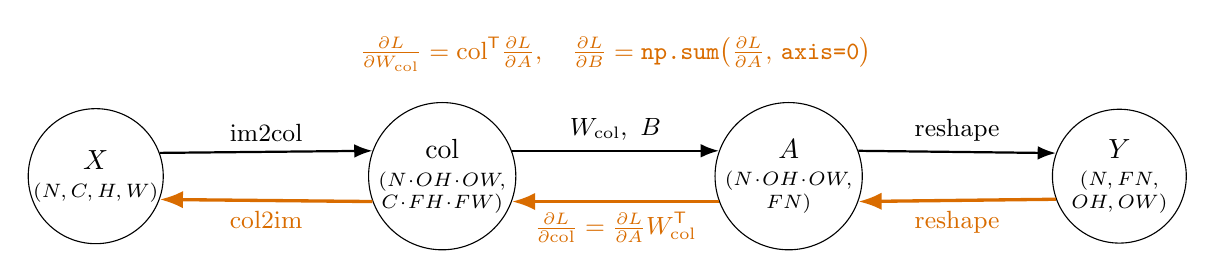
\begin{tikzpicture}[>=Latex,
  var/.style={draw,circle,minimum size=17mm,align=center,inner sep=0pt},
  bw/.style={<-,very thick,orange!85!black},
  bl/.style={orange!85!black,font=\small,align=center}]
\node[var] (X) at (0,0) {$X$\\[-2pt]{\scriptsize $(N,C,H,W)$}};
\node[var] (col) at (4.4,0) {col\\[-2pt]{\scriptsize $(N\!\cdot\!OH\!\cdot\!OW,$}\\[-4pt]{\scriptsize $C\!\cdot\!FH\!\cdot\!FW)$}};
\node[var] (A) at (8.8,0) {$A$\\[-2pt]{\scriptsize $(N\!\cdot\!OH\!\cdot\!OW,$}\\[-4pt]{\scriptsize $FN)$}};
\node[var] (Y) at (13.0,0) {$Y$\\[-2pt]{\scriptsize $(N,FN,$}\\[-4pt]{\scriptsize $OH,OW)$}};
\draw[->,thick] (X.20) -- node[above,font=\small] {im2col} (col.160);
\draw[->,thick] (col.20) -- node[above,font=\small] {$W_{\text{col}},\ B$} (A.160);
\draw[->,thick] (A.20) -- node[above,font=\small] {reshape} (Y.160);
\draw[bw] (X.-20) -- node[below,bl] {col2im} (col.-160);
\draw[bw] (col.-20) -- node[below,bl] {$\pd{L}{\text{col}}=\pd{L}{A}W_{\text{col}}\T$} (A.-160);
\draw[bw] (A.-20) -- node[below,bl] {reshape} (Y.-160);
\node[bl] at (6.6,1.55) {$\pd{L}{W_{\text{col}}}=\text{col}\T\pd{L}{A},\quad \pd{L}{B}=\texttt{np.sum}\bigl(\pd{L}{A},\,\texttt{axis=0}\bigr)$};
\end{tikzpicture}
\end{adjustbox}
\raggedright
\small
\begin{itemize}
\item \textbf{reshape}의 역전파: gradient의 모양만 원래대로 (값은 그대로)
\item \textbf{가운데는 Affine 계층}: $\pd{L}{W}=X\T\pd{L}{A}$, \ $\pd{L}{B}=\sum_{\text{행}}\pd{L}{A}$, \ $\pd{L}{X}=\pd{L}{A}W\T$ 그대로
\item \textbf{im2col}의 역전파 = \textbf{col2im}: 입력의 한 값이 col의 여러 행에 복사되었으므로 gradient를 \textbf{모두 더한다}\\
(im2col의 \texttt{=} 대신 col2im은 \texttt{+=}; 다변수 연쇄법칙 — 배치 정규화와 같은 원리)
\end{itemize}
\end{frame}

\begin{frame}{풀링 계층 구현하기}
\centering
\begin{adjustbox}{scale=1.3,max width=\linewidth}
\begin{tikzpicture}
\fill[orange!30] (0,0) rectangle ({2*\cellsz},{-2*\cellsz});
\fill[blue!15] ({2*\cellsz},0) rectangle ({4*\cellsz},{-2*\cellsz});
\fill[green!20] (0,{-2*\cellsz}) rectangle ({2*\cellsz},{-4*\cellsz});
\fill[black!10] ({2*\cellsz},{-2*\cellsz}) rectangle ({4*\cellsz},{-4*\cellsz});
\numgrid{0}{0}{4}{1,2,1,0,0,1,2,3,3,0,1,2,2,4,0,1}
\node[font=\small] at (2.9,-1) {$\xrightarrow{\text{전개}}$};
\fill[orange!30] (3.6,0) rectangle ++({4*\cellsz},-\cellsz);
\fill[blue!15] (3.6,-\cellsz) rectangle ++({4*\cellsz},-\cellsz);
\fill[green!20] (3.6,{-2*\cellsz}) rectangle ++({4*\cellsz},-\cellsz);
\fill[black!10] (3.6,{-3*\cellsz}) rectangle ++({4*\cellsz},-\cellsz);
\numgrid{3.6}{0}{4}{1,2,0,1,1,0,2,3,3,0,2,4,1,2,0,1}
\node[font=\small] at (6.4,-1) {$\xrightarrow{\text{max}}$};
\numgrid{7.2}{0}{1}{2,3,4,2}
\node[font=\small] at (8.4,-1) {$\xrightarrow{\text{reshape}}$};
\numgrid{9.3}{-0.5}{2}{2,3,4,2}
\end{tikzpicture}
\end{adjustbox}
\raggedright
\vskip4mm
\begin{itemize}
\item 풀링도 im2col로 입력을 전개
\item 풀링은 \textbf{채널마다 독립적} $\to$ 한 행이 ``한 채널의 한 윈도우''가 되도록 다시 \texttt{reshape}
\item 행마다 최댓값을 구한 뒤 모양을 되돌린다
\end{itemize}
\end{frame}

\begin{frame}[fragile]{\texttt{Pooling.forward}와 풀링의 역전파}
\begin{lstlisting}
    def forward(self, X):
        N, C, H, W = X.shape
        OH = output_size(H, self.PH, self.stride, self.pad)
        OW = output_size(W, self.PW, self.stride, self.pad)
        col = im2col(X, self.PH, self.PW, self.stride, self.pad)
        col = col.reshape(-1, self.PH * self.PW)           # one window per row
        self.argmax = np.argmax(col, axis=1)               # where the maximum was
        self.X_shape = X.shape
        Y = np.max(col, axis=1)
        return Y.reshape(N, OH, OW, C).transpose(0, 3, 1, 2)   # (N, C, OH, OW)
\end{lstlisting}
\small
\begin{itemize}
\item $y=\max(x_1,x_2,x_3,x_4)$에서 최댓값이 $x_k$이면 $\pd{y}{x_k}=1$, 나머지는 $0$
\item \textbf{최댓값이었던 원소에만} gradient를 그대로 전달, 나머지에는 $0$ (ReLU의 \texttt{mask}와 같다)
\item 그래서 순전파에서 최댓값의 위치 \texttt{argmax}를 기억해 둔다 (\texttt{backward}: \texttt{dcol[arange, argmax] = dY} $\to$ col2im)
\item 최댓값이 여러 개로 같으면: \texttt{np.argmax}가 고른 첫 위치로 보낸다
\end{itemize}
\end{frame}

\begin{frame}[fragile]{Flatten 계층}
\begin{itemize}
\item 합성곱·풀링을 거친 4차원 데이터를 Affine 계층에 넣으려면 데이터마다 한 줄로 펼쳐야 한다
\item 이것을 계층 하나로 (PyTorch의 \texttt{nn.Flatten}); 역전파는 모양을 되돌리는 것뿐
\end{itemize}
\begin{lstlisting}
class Flatten:
    """(N, C, H, W) -> (N, C*H*W) before an Affine layer (nn.Flatten in PyTorch)"""
    def forward(self, X):
        self.X_shape = X.shape
        return X.reshape(X.shape[0], -1)

    def backward(self, dY):
        return dY.reshape(self.X_shape)
\end{lstlisting}
\end{frame}

% =================================================
\section{CNN 구현하기}
% =================================================

\begin{frame}{SimpleConvNet의 구조}
\centering
\begin{adjustbox}{max width=\linewidth,max totalheight=3.0cm}
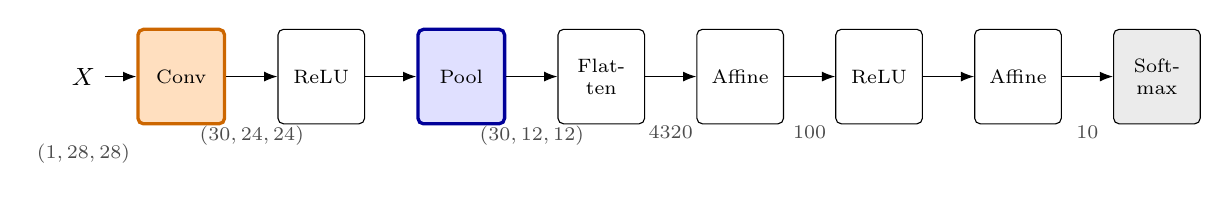
\begin{tikzpicture}[>=Latex,
  lay/.style={draw,rounded corners=2pt,minimum width=11mm,minimum height=12mm,
              font=\scriptsize,align=center,inner sep=1pt},
  cv/.style={lay,fill=orange!25,draw=orange!80!black,very thick},
  pl/.style={lay,fill=blue!12,draw=blue!60!black,very thick},
  sh/.style={font=\scriptsize,align=center,text=black!70},
  node distance=6.5mm]
\node[font=\small] (in) {$X$};
\node[cv,right=4mm of in] (c1) {Conv};
\node[lay,right=of c1] (r1) {ReLU};
\node[pl,right=of r1] (p1) {Pool};
\node[lay,right=of p1] (f1) {Flat-\\ten};
\node[lay,right=of f1] (a1) {Affine};
\node[lay,right=of a1] (r2) {ReLU};
\node[lay,right=of r2] (a2) {Affine};
\node[lay,right=of a2,fill=black!8] (sm) {Soft-\\max};
\draw[->] (in) -- (c1);
\draw[->] (c1) -- node[sh,below=5mm] {$(30,24,24)$} (r1);
\draw[->] (r1) -- (p1);
\draw[->] (p1) -- node[sh,below=5mm] {$(30,12,12)$} (f1);
\draw[->] (f1) -- node[sh,below=5mm] {$4320$} (a1);
\draw[->] (a1) -- node[sh,below=5mm] {$100$} (r2);
\draw[->] (r2) -- (a2);
\draw[->] (a2) -- node[sh,below=5mm] {$10$} (sm);
\node[sh,below=5mm] at (in.south) {$(1,28,28)$};
\end{tikzpicture}
\end{adjustbox}
\figcap{SimpleConvNet의 구조와 각 계층을 지난 뒤 데이터 하나의 shape}
\raggedright
\vskip1mm
\begin{itemize}
\item 지난 시간의 \texttt{MultiLayerNet}과 같은 방식
\item 매개변수는 \texttt{params} 딕셔너리, 같은 배열을 계층에도 넘김 $\to$ optimizer가 갱신하면 계층 가중치도 바뀜
\item 초깃값 \texttt{weight\_init\_std}: \texttt{"he"}이면 He ($C\cdot FH\cdot FW=25$ $\to$ $\sqrt{2/25}$), 숫자이면 그 표준편차
\item 계층이 모두 같은 \texttt{forward}/\texttt{backward} 형식 $\to$ 새 계층이 들어와도 network 코드는 그대로
\end{itemize}
\end{frame}

\begin{frame}{SimpleConvNet의 계층별 shape과 매개변수 수}
\centering
\small
\begin{tabular}{@{}llcr@{}}
\toprule
계층 & 설정 & 출력 shape & 매개변수 수 \\
\midrule
입력 & & $(1,28,28)$ & \\
Conv & $5\times5$ 필터 $30$개 & $(30,24,24)$ & $30\cdot1\cdot5\cdot5+30=780$ \\
ReLU & & $(30,24,24)$ & \\
Pooling & $2\times2$ 최대 풀링 & $(30,12,12)$ & \\
Flatten & & $4320$ & \\
Affine & & $100$ & $4320\cdot100+100=432100$ \\
ReLU & & $100$ & \\
Affine & & $10$ & $100\cdot10+10=1010$ \\
\midrule
합계 & & & $433890$ \\
\bottomrule
\end{tabular}
\figcap{합성곱은 스트라이드 $1$, 패딩 $0$; 풀링은 스트라이드 $2$; 출력 shape은 데이터 하나의 것}
\raggedright
\begin{itemize}
\item 합성곱 계층의 매개변수는 $\mathbf{780}$개뿐, 매개변수의 $99.6\%$는 첫 번째 Affine 계층에 (가중치 공유 덕분)
\end{itemize}
\end{frame}

\begin{frame}{gradient 확인과 MNIST 학습 설정}
\begin{itemize}
\item \textbf{gradient 확인} (\texttt{conv\_basics.py}의 (3))
  \begin{itemize}
  \item 작은 SimpleConvNet: 입력 $(2,8,8)$, $3\times3$ 필터 $3$개, 데이터 $5$개
  \item W1 $(3,2,3,3)$, B1, W2 $(27,5)$, B2, W3 $(5,4)$, B3 모두 $\max|\text{backprop}-\text{numerical}|\approx10^{-9}$
  \item 합성곱, 풀링, Flatten을 지나는 역전파가 모두 올바르다
  \end{itemize}
\item \textbf{MNIST로 학습하기} (\texttt{mnist\_cnn.py})
  \begin{itemize}
  \item SimpleConvNet ($5\times5$ 필터 $30$개, 은닉 $100$)을 Adam (학습률 $0.001$, 미니배치 $100$)으로 $10$ epoch
  \item 초깃값은 표준편차 $0.01$로 작게 시작 $\to$ 학습으로 생긴 필터의 무늬가 잘 드러난다
  \item 비교: 지난 시간의 MLP ($784\to100\to10$, He 초깃값)를 같은 조건으로
  \end{itemize}
\end{itemize}
\end{frame}

\begin{frame}{학습 결과: SimpleConvNet vs. MLP}
\centering
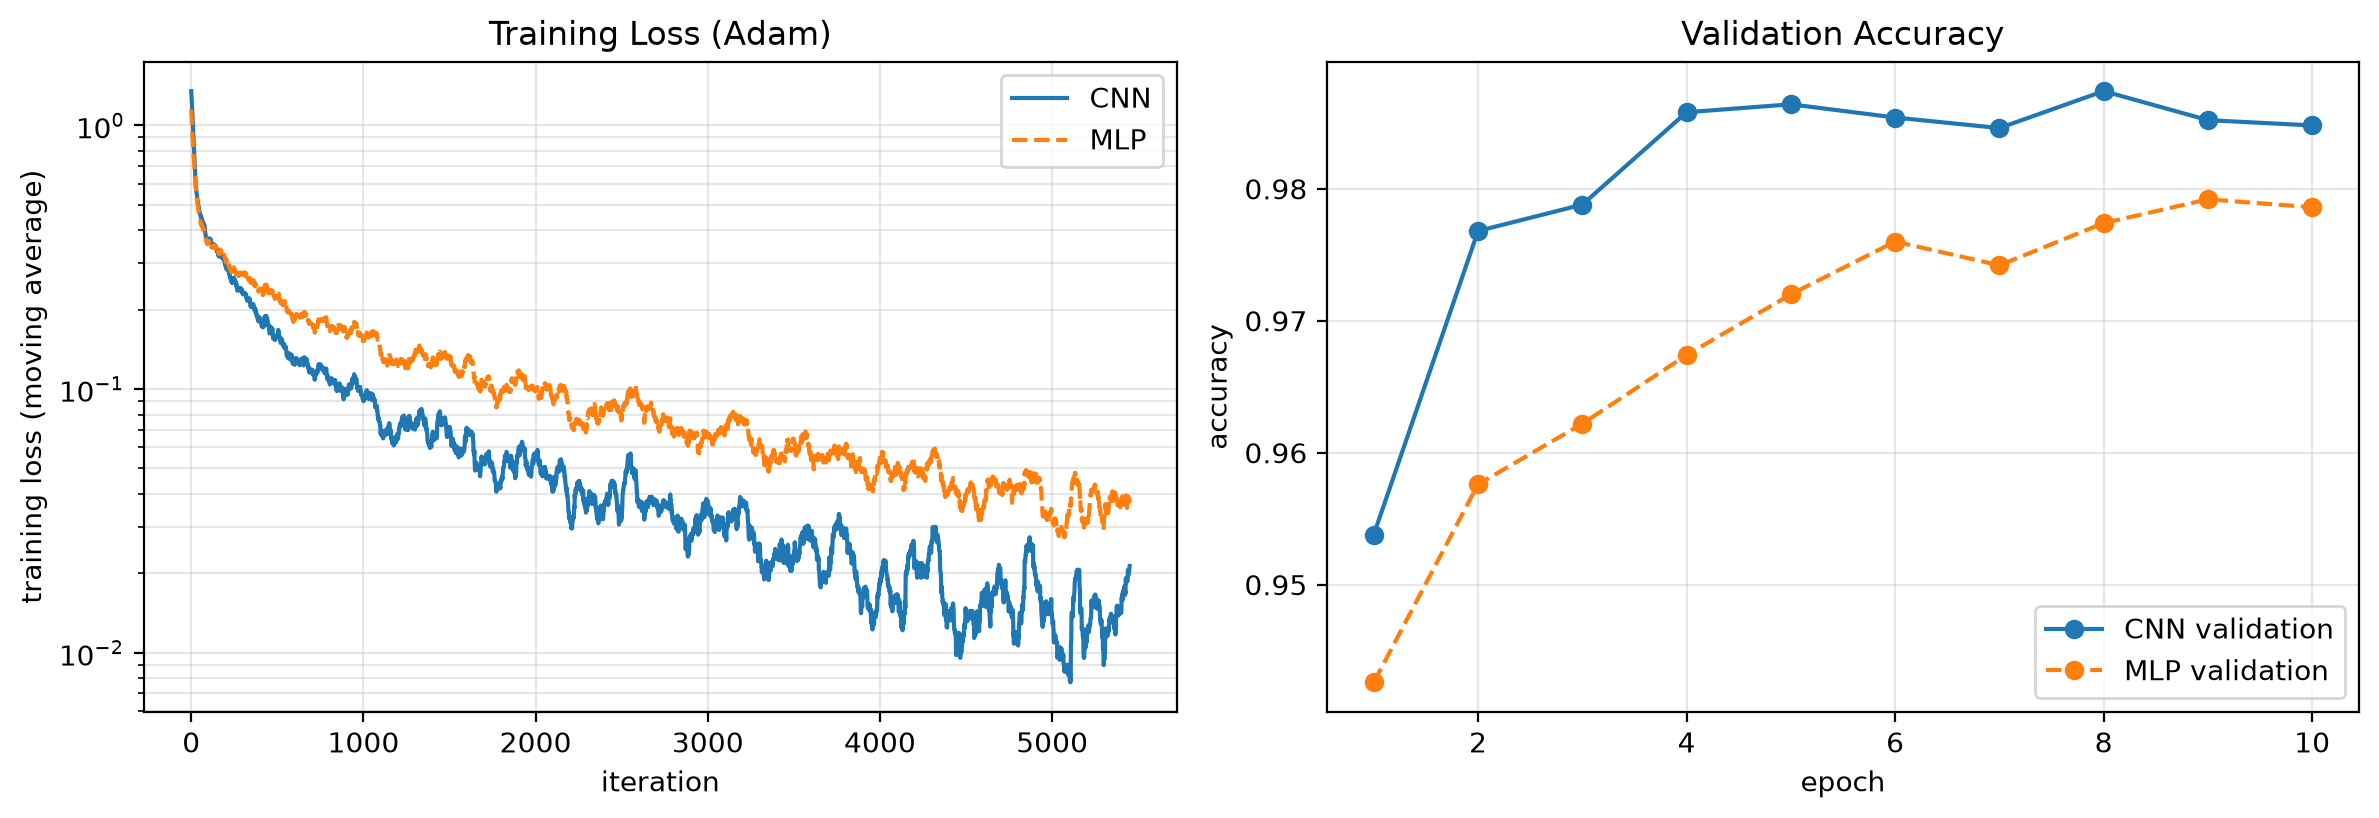
\includegraphics[width=\linewidth]{figures/cnn_mnist.png}
\figcap{훈련 손실 (50 iteration 이동평균, 로그 눈금, 왼쪽)과 epoch별 검증 정확도 (오른쪽)}
\end{frame}

\begin{frame}{학습 결과 비교}
\centering
\footnotesize
\begin{tabular}{@{}lccccccc@{}}
\toprule
& \multicolumn{4}{c}{검증 정확도} & & & \\
\cmidrule(lr){2-5}
& 1 epoch & 2 epoch & 5 epoch & 10 epoch & 시험 & 매개변수 & epoch당 \\
\midrule
SimpleConvNet & $95.4\%$ & $97.7\%$ & $98.6\%$ & $98.5\%$ & $\mathbf{98.5\%}$ & $433890$ & 약 $60$초 \\
MLP ($784\to100\to10$) & $94.3\%$ & $95.8\%$ & $97.2\%$ & $97.9\%$ & $97.6\%$ & $79510$ & 약 $1$초 \\
\bottomrule
\end{tabular}
\raggedright
\vskip2mm
\begin{itemize}
\small
\item CNN은 \textbf{$2$ epoch 만에} $97.7\%$ $\approx$ MLP의 $10$ epoch $97.9\%$; 시험 오류 $237\to154$장 (약 $35\%$ 감소)
\item 손실도 CNN이 훨씬 빨리, 훨씬 낮게 내려간다
\item 매개변수 수가 달라 공정한 비교는 아님 — 합성곱 계층의 $780$개 매개변수가 \textbf{좋은 특징}을 만들어 뒤의 Affine 계층의 분류를 쉽게 한다
\item numpy CNN은 epoch당 약 $1$분 $\to$ GPU와 최적화된 라이브러리가 중요 ($20$ epoch이면 시험 약 $99\%$)
\end{itemize}
\end{frame}

% =================================================
\section{CNN 시각화하기}
% =================================================

\begin{frame}{첫 번째 층의 가중치 시각화하기}
\centering
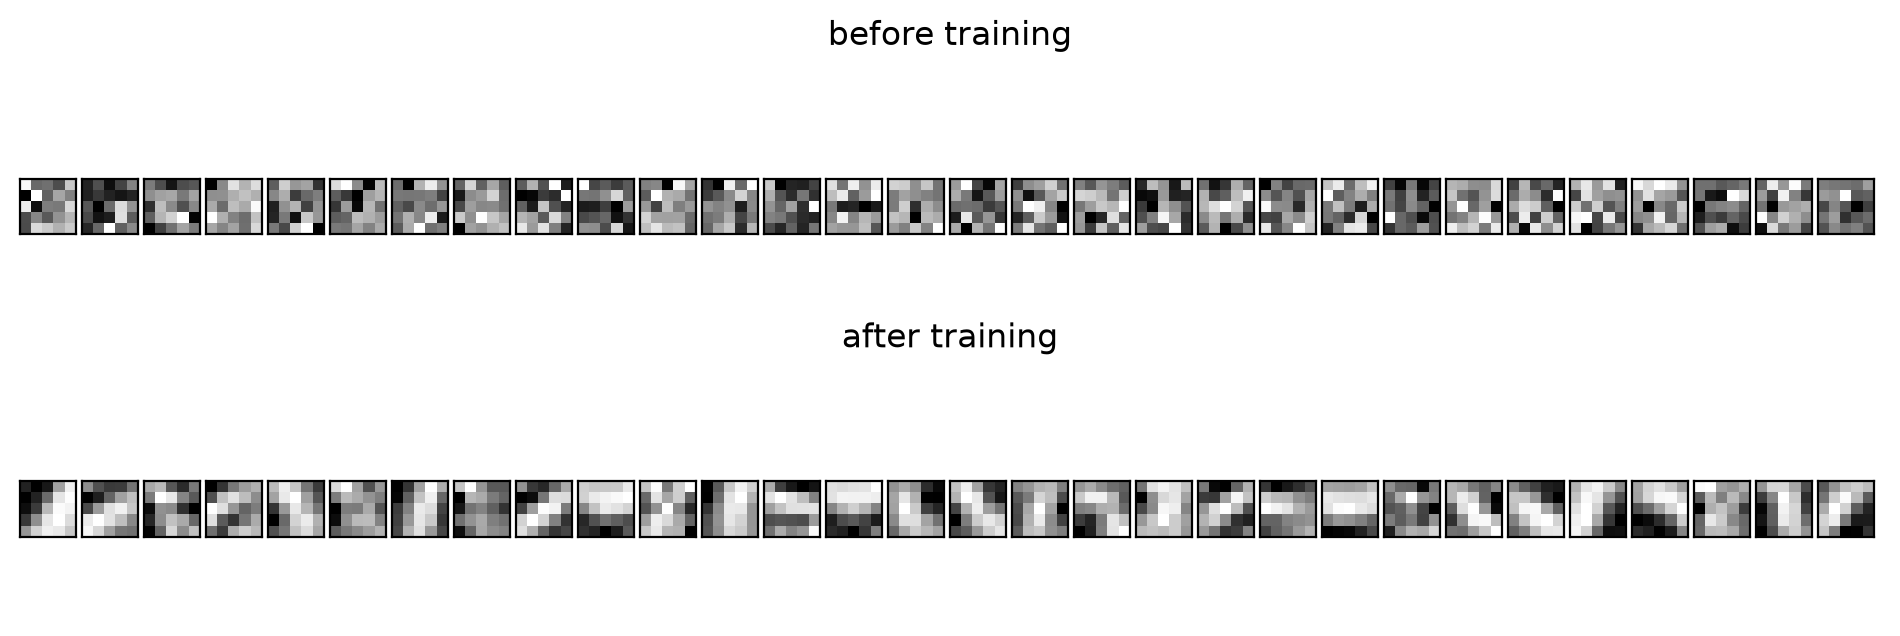
\includegraphics[width=0.78\linewidth]{figures/cnn_filters.png}
\figcap{첫 번째 합성곱 계층의 필터 $30$개 $(30,1,5,5)$: 학습 전 (위)과 학습 후 (아래), 밝을수록 큰 가중치}
\raggedright
\footnotesize
\begin{itemize}
\item 학습 전: 무작위 $\to$ 학습 후: 흰색과 검은색이 \textbf{규칙적으로 나뉜} 모양
\item 세로 경계, 가로 경계, 대각선 띠 $\to$ \textbf{에지}에 반응하는 필터
\item Sobel처럼 사람이 설계했던 필터를 network가 데이터로부터 \textbf{스스로} 찾아냈다
\end{itemize}
\end{frame}

\begin{frame}{필터는 무엇에 반응하는가: 특징 맵}
\centering
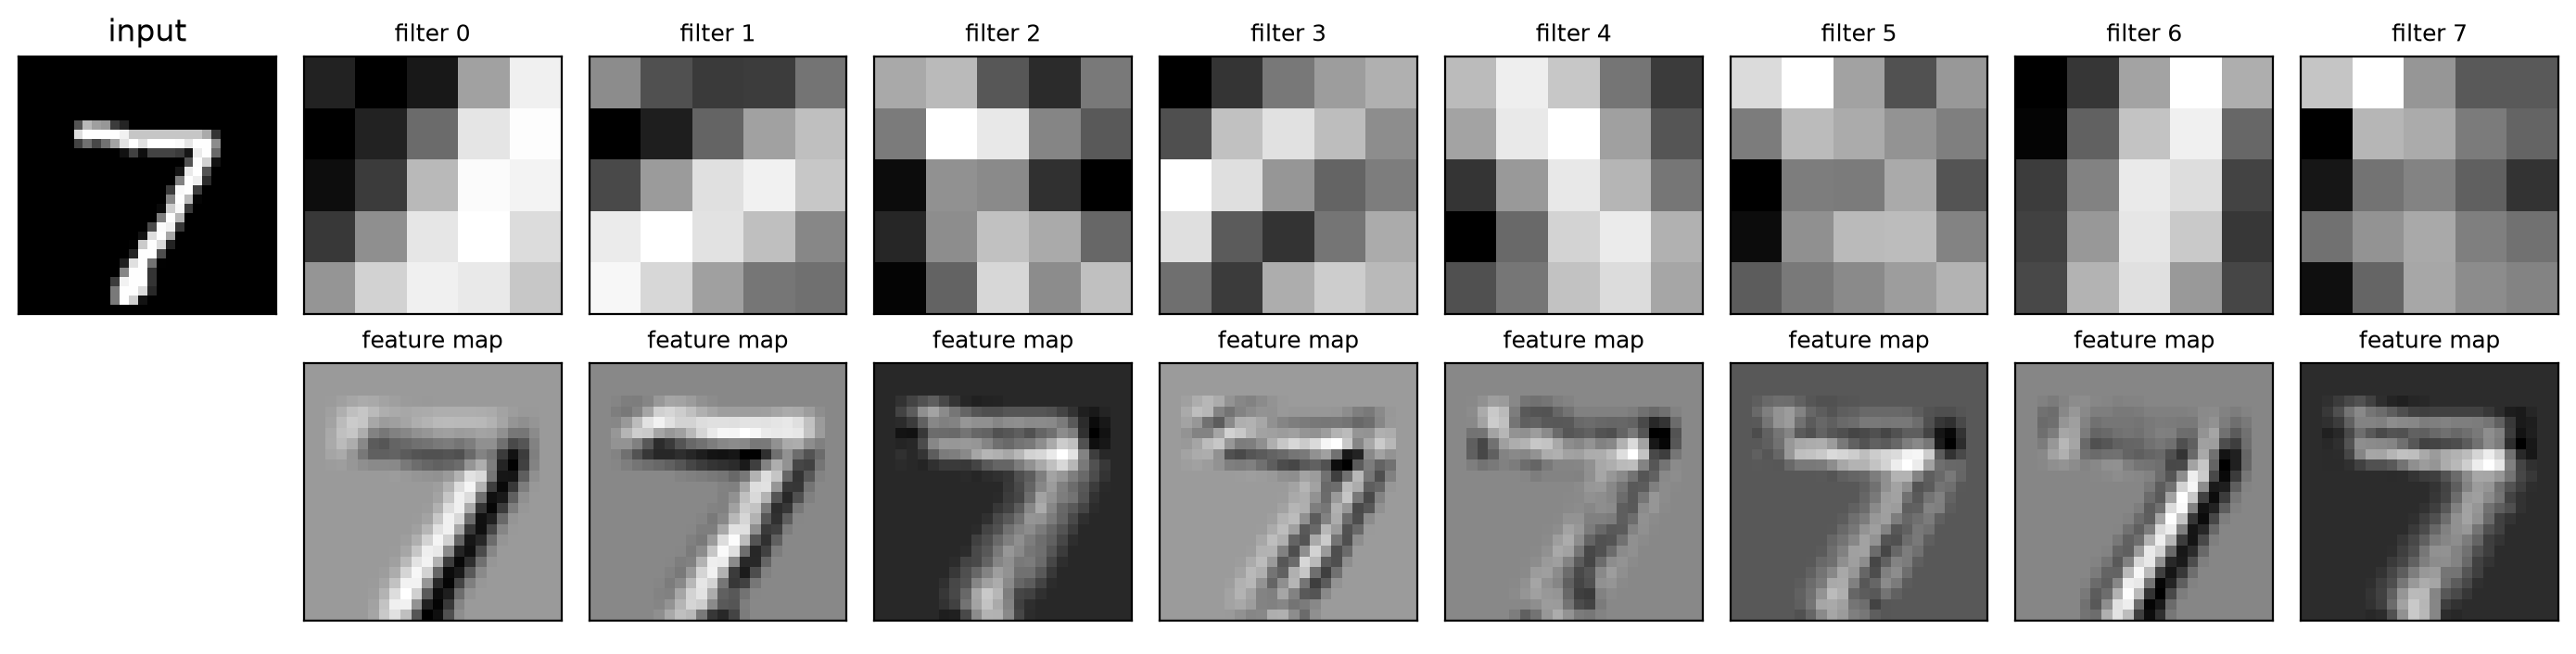
\includegraphics[width=0.93\linewidth]{figures/cnn_feature_maps.png}
\figcap{입력 이미지와 학습된 필터 $8$개 (위), 각 필터의 출력 특징 맵 (아래, ReLU 적용 전): \texttt{cnn.layers[0].forward(image)} $\to (1,30,24,24)$}
\raggedright
\small
\begin{itemize}
\item 특징 맵마다 숫자 7의 \textbf{서로 다른 부분이 밝게}: 필터 $0$은 대각선 획의 가장자리, 필터 $1$은 위쪽 가로 획의 아래 가장자리, 필터 $6$은 대각선 획 자체
\item 첫 층의 필터는 특정 방향의 \textbf{에지}에 반응 — 모든 위치에 적용되므로 어디에 있든 찾는다
\item $30$장의 특징 맵을 풀링으로 줄인 뒤 Affine 계층이 조합하여 숫자를 판단
\end{itemize}
\end{frame}

\begin{frame}{층 깊이에 따른 추출 정보 변화}
\centering
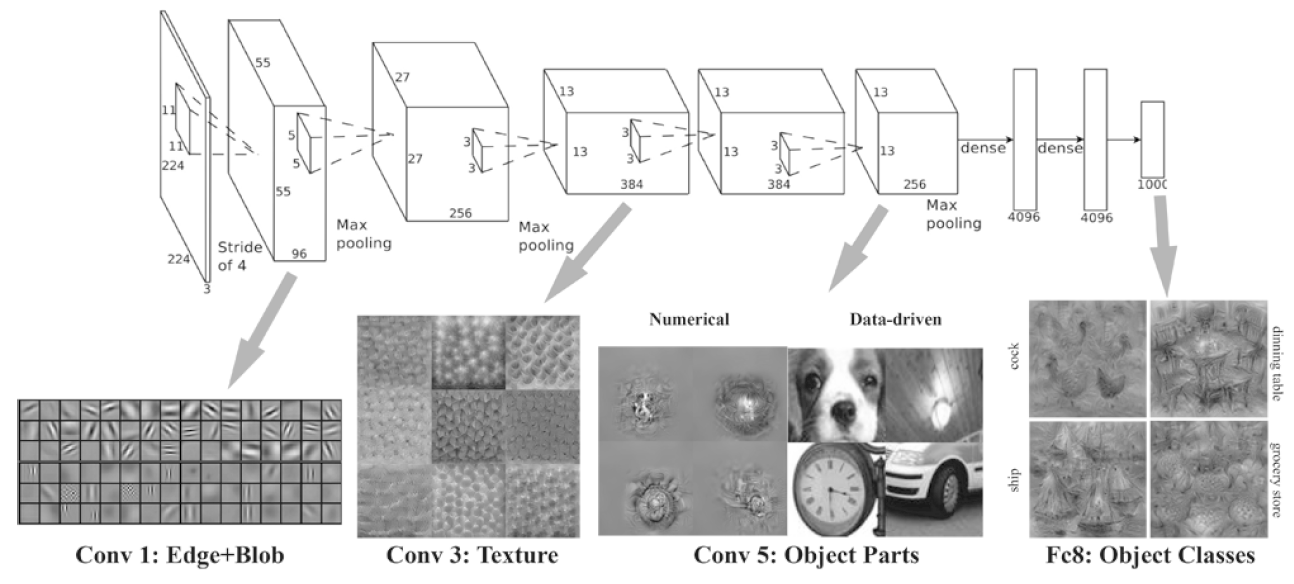
\includegraphics[width=0.9\linewidth]{figures/cnn_depth_layers.png}
\figcap{ImageNet으로 학습한 $8$층 CNN (AlexNet)의 각 층 뉴런이 강하게 반응하는 이미지}
\end{frame}

\begin{frame}{층이 깊어질수록: 단순한 모양 $\to$ 의미}
\small
\begin{itemize}
\item \textbf{Conv 1}: 에지와 블롭 (Sobel 같은 방향 필터)
\item \textbf{Conv 3}: 텍스처 (벌집, 비늘 같은 반복 무늬)
\item \textbf{Conv 5}: 사물의 일부 (개 얼굴, 시계, 바퀴)
  \begin{itemize}
  \item Numerical: 뉴런 출력이 최대가 되도록 계산으로 만든 입력
  \item Data-driven: 실제 데이터 중 가장 강하게 반응한 이미지
  \end{itemize}
\item \textbf{Fc8}: 사물의 클래스 (닭, 식탁, 배, 식료품점)
\item 층이 깊어질수록 단순한 모양 $\to$ ``고급'' 정보, 즉 사물의 \textbf{의미}에 반응한다
\end{itemize}
\vskip2mm
\textbf{층을 깊게 쌓는 이유}
\begin{itemize}
\item \textbf{단순한 특징을 조합하여 점점 추상적인 특징을 만드는 것} = 층을 깊게 쌓는 이유
\item 합성곱을 거듭할수록 출력 한 원소의 \textbf{수용 영역}(receptive field)이 넓어진다 $\to$ 뒤쪽 층은 넓은 영역을 보고 판단
\item 고양이 그림 (1절)의 ``에지 $\to$ 부분 $\to$ 전체''를 실제 network가 데이터로부터 스스로 만든다
\end{itemize}
\end{frame}

\begin{frame}{뒤쪽 층으로 갈수록 넓어지는 수용 영역}
\centering
\begin{adjustbox}{max width=\linewidth,max totalheight=4.6cm}
\begin{tikzpicture}[>=Latex,x=0.62cm,y=1.15cm,
  nd/.style={circle,draw=black!45,fill=white,minimum size=4.2mm,inner sep=0pt},
  hn/.style={circle,draw=orange!80!black,fill=orange!35,very thick,minimum size=4.2mm,inner sep=0pt}]
% (a) 1D: 3 conv layers (filter 3, stride 1) on 9 inputs
\foreach \l in {0,1,2,3} {
  \pgfmathtruncatemacro{\lo}{\l}
  \pgfmathtruncatemacro{\hi}{8-\l}
  \foreach \x in {\lo,...,\hi} {
    \pgfmathtruncatemacro{\d}{abs(\x-4)}
    \pgfmathtruncatemacro{\r}{3-\l}
    \ifnum\d>\r \node[nd] (n\l-\x) at (\x,\l) {}; \else \node[hn] (n\l-\x) at (\x,\l) {}; \fi
  }
}
\foreach \l in {1,2,3} {
  \pgfmathtruncatemacro{\m}{\l-1}
  \pgfmathtruncatemacro{\lo}{\l}
  \pgfmathtruncatemacro{\hi}{8-\l}
  \foreach \x in {\lo,...,\hi} {
    \pgfmathtruncatemacro{\d}{abs(\x-4)}
    \pgfmathtruncatemacro{\r}{3-\l}
    \pgfmathtruncatemacro{\xa}{\x-1}
    \pgfmathtruncatemacro{\xb}{\x+1}
    \ifnum\d>\r
      \foreach \u in {\xa,\x,\xb} \draw[black!20] (n\m-\u) -- (n\l-\x);
    \else
      \foreach \u in {\xa,\x,\xb} \draw[orange!80!black,thick] (n\m-\u) -- (n\l-\x);
    \fi
  }
}
\foreach \l/\t in {0/입력,1/층 $1$,2/층 $2$,3/층 $3$} \node[font=\small,anchor=east] at (-0.6,\l) {\t};
\foreach \l/\w in {1/3,2/5,3/7} \node[font=\small,anchor=west,text=orange!60!black] at (8.6,\l) {보는 입력: $\w$칸};
\draw[decorate,decoration={brace,mirror,amplitude=5pt},thick] (0.7,-0.35) -- (7.3,-0.35)
  node[midway,below=6pt,font=\small] {층 $3$의 한 원소가 보는 입력: $7$칸};
\node[font=\small] at (4,-1.45) {(a) 필터 길이 $3$인 합성곱을 세 번 (1차원)};
% (b) 2D: nested receptive fields on a 9x9 input
\begin{scope}[shift={(13.6,-0.55)},x=0.42cm,y=0.42cm]
\fill[orange!12] (1,1) rectangle (8,8);
\fill[orange!28] (2,2) rectangle (7,7);
\fill[orange!55] (3,3) rectangle (6,6);
\draw[step=1,black!25] (0,0) grid (9,9);
\draw[orange!80!black,very thick] (3,3) rectangle (6,6);
\draw[orange!80!black,very thick,dashed] (2,2) rectangle (7,7);
\draw[orange!80!black,very thick,dotted] (1,1) rectangle (8,8);
\draw[black!60] (0,0) rectangle (9,9);
\draw (6,4.5) -- (10.3,7.5) node[right,font=\small] {층 $1$: $3\times3$};
\draw (7,3.5) -- (10.3,4.5) node[right,font=\small] {층 $2$: $5\times5$};
\draw (8,2.5) -- (10.3,1.5) node[right,font=\small] {층 $3$: $7\times7$};
\node[font=\small] at (6.3,-2.5) {(b) 같은 일을 이미지 (2차원)에서};
\end{scope}
\end{tikzpicture}
\end{adjustbox}
\raggedright
\vskip2mm
\small
\begin{itemize}
\item 층 $3$의 원소 하나 (맨 위 주황색)는 입력 $7$칸에 의존한다
\item $3\times3$ 필터 (스트라이드 $1$)를 $L$번 쌓으면 수용 영역은 $(2L+1)\times(2L+1)$
\item 중간에 $2\times2$ 풀링 (스트라이드 $2$)이 있으면 훨씬 빨리 넓어진다 $\to$ 뒤쪽 층은 이미지의 큰 부분이나 전체를 본다
\end{itemize}
\end{frame}

% =================================================
\section{대표적인 CNN}
% =================================================

\begin{frame}{CNN 이전의 문자 인식: 사람이 설계한 특징}
\begin{remarkbox}[CNN 이전의 문자 인식: 사람이 설계한 특징]
\small
1990년대까지의 주류: \textbf{``사람이 설계한 특징 추출기 + 학습하는 분류기''}
\begin{itemize}
\item \textbf{템플릿 매칭 (1950--60년대)}: 글자마다 표준 모양과 비교 (템플릿 = 큰 필터) — 위치·크기·글씨체에 약함. 기계 판독용 \textbf{전용 글꼴}도 등장 (광학식 OCR-A, 수표의 자기잉크식 E-13B)
\item \textbf{사람이 설계한 특징 (1960--90년대)}: 방향 필터(Sobel, Gabor)의 획의 양, zoning (사실상 평균 풀링), 구멍·끝점·교차점 개수, 모멘트 $\to$ k-NN, SVM 등
\item \textbf{한계}: 문자 체계마다 전문가가 특징을 새로 설계, 기울기·굵기에 약함, 버린 정보는 되살릴 수 없음
\end{itemize}
LeCun 등 (1998): \textbf{특징 추출기까지 데이터로 학습}하자. 학습된 첫 층 필터도 방향 에지 필터와 비슷해진다 — 어려웠던 것은 그 위의 \textbf{복잡한 조합}을 사람이 설계하는 일.
\end{remarkbox}
\end{frame}

\begin{frame}{LeNet (1998)}
\centering
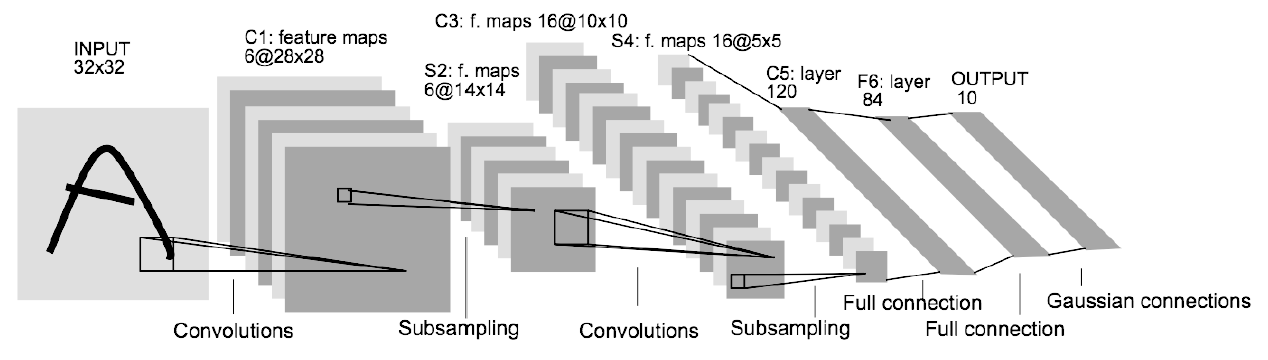
\includegraphics[width=0.9\linewidth]{figures/lenet.png}
\figcap{LeNet-5의 구조 (LeCun 등, 1998). ``$6@28\times28$''은 $28\times28$ 크기의 특징 맵 $6$장}
\raggedright
\footnotesize
\begin{itemize}
\item C = 합성곱, S = \textbf{서브샘플링} ($2\times2$ 합 $\times$ 학습 계수 $+$ 편향 $\to$ 활성화), F = 완전연결
\item C5: $5\times5$ 입력에 $5\times5$ 필터 $120$개 $\to$ $1\times1$ 출력 $120$개 (사실상 완전연결); 출력의 Gaussian connections $\to$ 지금은 Softmax
\item SimpleConvNet과 거의 같은 구조. 지금과 다른 점: sigmoid 계열 (scaled tanh) $\to$ \textbf{ReLU}, 서브샘플링 $\to$ \textbf{최대 풀링}
\item 거의 $30$년 전에 이미 지금의 CNN과 같은 기본 구조가 완성
\end{itemize}
\end{frame}

\begin{frame}{LeNet의 서브샘플링}
\begin{remarkbox}[LeNet의 서브샘플링]
\footnotesize
서브샘플링 = ``표본을 줄인다'' (해상도를 낮춘다): LeNet의 풀링 계층.
특징 맵마다 겹치지 않는 $2\times2$ 영역 하나 $\to$ 출력 하나:
\[
y=\sigma\bigl(w\,(x_1+x_2+x_3+x_4)+b\bigr)
\]
\vskip-2mm
\begin{itemize}
\item 네 값을 더하고, 학습하는 계수 $w$를 곱하고 편향 $b$를 더한 뒤 활성화 $\sigma$ (scaled tanh)
\item 예: $\begin{pmatrix}1&3\\2&6\end{pmatrix}$, $w=0.25$, $b=0$ $\to$ $0.25\times12=3$ = 네 값의 \textbf{평균}
\item 즉 \textbf{평균 풀링 (스트라이드 $2$)} + 학습하는 배율·편향 + 활성화; $28\times28\to14\times14$
\item 매개변수: 특징 맵마다 $w$, $b$ 하나씩 (위치 공유) $\to$ S2 $12$개, S4 $32$개 (최대 풀링은 $0$개)
\item 목적: 획의 위치가 조금 달라도 출력이 거의 같게 $\to$ 복합 세포, Neocognitron의 C층과 같은 역할
\end{itemize}
\end{remarkbox}
\end{frame}

\begin{frame}{AlexNet (2012)}
\centering
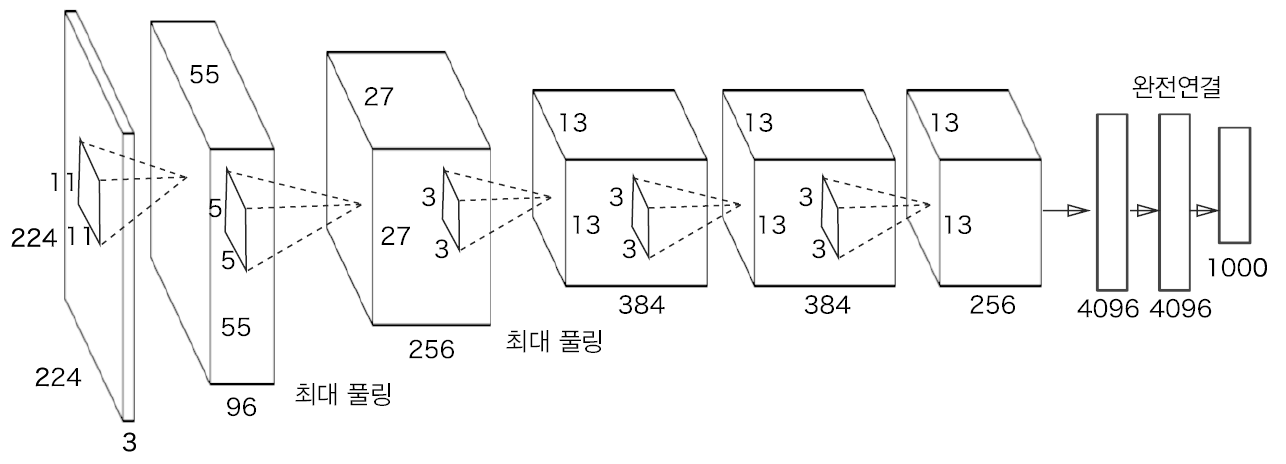
\includegraphics[width=0.78\linewidth]{figures/alexnet.png}
\figcap{AlexNet의 구조 (Krizhevsky 등, 2012): 합성곱 계층 $5$개와 완전연결 계층 $3$개}
\raggedright
\footnotesize
\begin{itemize}
\item ILSVRC 2012 top-5 오류율 약 $15\%$ (2위 $26\%$) $\to$ 딥러닝 열풍
\item LeNet과 같은 큰 틀 + 변화: \textbf{ReLU}, \textbf{LRN} (국소적 정규화, 지금은 배치 정규화), \textbf{드롭아웃}, \textbf{최대 풀링}
\item 매개변수 약 $6000$만 개 $\Leftarrow$ \textbf{빅데이터} (ImageNet, 약 $120$만 장)와 \textbf{GPU} 덕분에 학습 가능
\item 입력은 원 논문대로 $224$로 표기; 출력 $55$는 입력 $227$, 패딩 $0$일 때 공식과 맞는다 (연습문제 1)
\end{itemize}
\end{frame}

\begin{frame}{AlexNet에는 지금까지 배운 부품이 모두 있다}
\begin{keybox}[AlexNet에는 지금까지 배운 부품이 모두 있다]
\begin{itemize}
\item ReLU, 최대 풀링, 드롭아웃 (지난 주), 정규화 계층 (배치 정규화의 선배 격), GPU에서의 대규모 행렬곱 (im2col)
\item 그 뒤의 CNN도 같은 부품을 \textbf{더 깊게} 쌓는 방향으로 발전
  \begin{itemize}
  \item \textbf{VGG} (2014): $3\times3$ 합성곱을 쌓아 $16\sim19$층 (완전연결 계층 포함)
  \item \textbf{GoogLeNet} (2014): 여러 크기의 필터를 병렬로
  \item \textbf{ResNet} (2015): 입력을 건너뛰어 더하는 skip connection으로 $150$층 이상
  \end{itemize}
\end{itemize}
\end{keybox}
\end{frame}

% =================================================
\section{PyTorch로 구현하기}
% =================================================

\begin{frame}{우리의 구현과 PyTorch}
\begin{itemize}
\item 지난 시간의 PyTorch 완전연결 network와 같은 방법 $\to$ 바뀌는 것은 \textbf{계층의 이름}뿐 (\texttt{mnist\_cnn\_torch.py})
\end{itemize}
\vskip2mm
\centering
\footnotesize
\begin{tabular}{@{}ll@{}}
\toprule
우리의 구현 (\texttt{conv\_layers.py}) & PyTorch \\
\midrule
\texttt{Convolution(W, B, stride, pad)} & \texttt{nn.Conv2d(C, FN, kernel\_size, stride, padding)} \\
\texttt{Pooling(2, 2)} & \texttt{nn.MaxPool2d(2)} \\
\texttt{Flatten()} & \texttt{nn.Flatten()} \\
필터 \texttt{W}: $(FN,C,FH,FW)$ & \texttt{weight}: $(FN,C,FH,FW)$ (같은 순서) \\
\bottomrule
\end{tabular}
\raggedright
\vskip3mm
\begin{itemize}
\item 데이터는 $(N,1,28,28)$ 모양의 텐서로 (\texttt{to\_dataset}: \texttt{reshape(-1, 1, 28, 28)}, one-hot $\to$ 클래스 번호)
\item 학습 루프는 지난 시간의 코드와 같다
\end{itemize}
\end{frame}

\begin{frame}[fragile]{PyTorch 모델 정의}
\begin{lstlisting}[basicstyle=\ttfamily\small]
model = nn.Sequential(
    nn.Conv2d(1, 30, kernel_size=5),      # (N, 1, 28, 28) -> (N, 30, 24, 24)
    nn.ReLU(),
    nn.MaxPool2d(2),                      # -> (N, 30, 12, 12)
    nn.Flatten(),                         # -> (N, 4320)
    nn.Linear(30 * 12 * 12, 100),
    nn.ReLU(),
    nn.Linear(100, 10),
).to(device)
\end{lstlisting}
\begin{itemize}
\item SimpleConvNet과 똑같은 구조: Conv $\to$ ReLU $\to$ Pool $\to$ Flatten $\to$ Affine $\to$ ReLU $\to$ Affine
\item 주석의 shape 변화가 계층별 출력 shape 표와 같다; \texttt{.to(device)}로 CPU/GPU 선택
\end{itemize}
\end{frame}

\begin{frame}{numpy 구현과 PyTorch의 비교}
\centering
\small
\begin{tabular}{@{}lcccccc@{}}
\toprule
& \multicolumn{4}{c}{검증 정확도} & & \\
\cmidrule(lr){2-5}
& 1 epoch & 2 epoch & 5 epoch & 10 epoch & 시험 & epoch당 \\
\midrule
numpy (\texttt{conv\_layers.py}) & $95.4\%$ & $97.7\%$ & $98.6\%$ & $98.5\%$ & $98.5\%$ & 약 $60$초 \\
PyTorch (CPU) & $97.6\%$ & $98.4\%$ & $98.6\%$ & $99.1\%$ & $98.8\%$ & 약 $12$초 \\
\bottomrule
\end{tabular}
\raggedright
\vskip3mm
\begin{itemize}
\item 같은 구조, 같은 optimizer $\to$ 결과가 비슷 (초깃값·미니배치 순서가 달라 똑같지는 않음)
\item 같은 CPU에서 PyTorch가 약 $5$배 빠름 (C++ 최적화 라이브러리); GPU가 있으면 \texttt{device="cuda"}만으로 더 빨라질 수 있음 (환경에 따라 다르니 실측)
\item \texttt{nn.Conv2d}의 기본 초깃값: 균등분포 ($\pm1/\sqrt{25}$)
\end{itemize}
\end{frame}

\begin{frame}{PyTorch로 학습한 첫 번째 층의 필터}
\centering
\vskip4mm
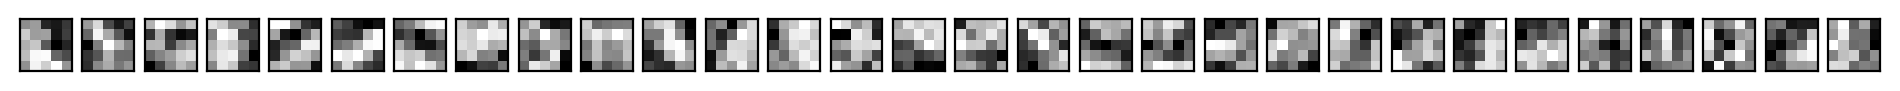
\includegraphics[width=\linewidth]{figures/cnn_torch_filters.png}
\figcap{PyTorch로 학습한 첫 번째 합성곱 계층의 필터 $30$개 (\texttt{model[0].weight})}
\raggedright
\vskip5mm
\begin{itemize}
\item \textbf{여러 방향의 에지} 모양 $\to$ 사람이 설계한 Sobel 필터와 닮은 필터를 데이터로부터 스스로 학습
\end{itemize}
\end{frame}

% =================================================
\section{정리}
% =================================================

\begin{frame}{합성곱 신경망: 정리}
\begin{keybox}[합성곱 신경망: 정리]
\small
\begin{itemize}
\item CNN = 지금까지의 신경망 + \textbf{합성곱 계층} + \textbf{풀링 계층}
\item 합성곱 계층은 이미지의 \textbf{형상을 유지}하며, 같은 필터를 모든 위치에 적용 (가중치 공유).
출력 크기 $OH=\lfloor\frac{H+2P-FH}{S}\rfloor+1$
\item 필터는 4차원 $(FN,C,FH,FW)$, 데이터는 4차원 $(N,C,H,W)$
\item 풀링 계층은 매개변수 없이 공간 크기를 줄이며, 작은 위치 변화에 강하다
\item \textbf{im2col}을 쓰면 합성곱은 하나의 행렬곱 = Affine 계층. 역전파는 Affine의 역전파와 col2im
\item 첫 층의 필터는 에지와 블롭에 반응하고, 층이 깊어질수록 더 추상적인 정보를 추출
\item LeNet (1998)과 AlexNet (2012)이 대표적인 CNN; 빅데이터와 GPU가 딥러닝 발전의 큰 원동력
\end{itemize}
\end{keybox}
\end{frame}

% =================================================
\section{연습문제}
% =================================================

\begin{frame}{연습문제 (1)}
\small
\begin{enumerate}
\item 출력 크기를 구하라. (a) 입력 $(32,32)$, 필터 $(5,5)$, $P=2$, $S=1$ \
(b) 입력 $(227,227)$, 필터 $(11,11)$, $P=0$, $S=4$ (AlexNet 첫 층) \
(c) $(28,28)$에 $2\times2$ 최대 풀링 (스트라이드 $2$) 두 번
\item 입력 $\begin{pmatrix}1&0&2&1\\0&3&1&0\\2&1&0&4\\1&0&1&2\end{pmatrix}$에
필터 $\begin{pmatrix}1&0\\0&-1\end{pmatrix}$ ($S=1$, $P=0$)를 적용한 결과를 손으로 계산하라. 같은 입력에 $2\times2$ 최대 풀링 ($S=2$, $P=0$)한 결과도 구하라.
\item RGB 이미지 ($C=3$)에 $3\times3$ 필터 $64$개인 합성곱 계층의 매개변수 수는?
입력 $(3,32,32)$, $P=1$일 때 같은 출력 $(64,32,32)$을 완전연결 계층으로 만들면 가중치는 몇 개?
\item 2번의 최대 풀링에서 출력 쪽 gradient가 $\begin{pmatrix}1&2\\3&4\end{pmatrix}$일 때, 입력 쪽 gradient ($4\times4$)를 구하라.
\end{enumerate}
\end{frame}

\begin{frame}{연습문제 (2)}
\small
\begin{enumerate}
\setcounter{enumi}{4}
\item 길이 $5$인 1차원 입력 $(x_1,\ldots,x_5)$에 길이 $3$인 필터 (스트라이드 $1$): im2col 행렬 ($3\times3$)을 쓰고,
$x_3$이 몇 번 등장하는지 세어 보라. col2im에서 gradient를 \textbf{더해야} 하는 이유를 설명하라.
\item SimpleConvNet의 합성곱 계층에 패딩 $2$를 주도록 고쳐 보라.
\texttt{conv\_out}, \texttt{pool\_out}, \texttt{flat}은 각각 얼마인가? \texttt{pad}를 넘기는 부분과 \texttt{flat}의 계산을 고친 뒤
\texttt{conv\_basics.py}의 gradient 확인으로 검증하라.
\item \texttt{mnist\_cnn\_torch.py}를 고쳐 LeNet과 비슷한 network를 만들고 학습시켜라:\\
Conv $5\times5$ $6$개 (패딩 $2$) $\to$ ReLU $\to$ MaxPool $\to$ Conv $5\times5$ $16$개 $\to$ ReLU $\to$ MaxPool $\to$ FC $120$ $\to$ ReLU $\to$ FC $84$ $\to$ ReLU $\to$ FC $10$.
각 계층 뒤의 shape을 표로 정리하고, 매개변수 수와 검증 정확도를 SimpleConvNet과 비교하라.
\end{enumerate}
\end{frame}

\end{document}
